\documentclass[a4paper, 12pt]{report}
\usepackage[table,xcdraw]{xcolor}
\usepackage[utf8]{inputenc}
\usepackage{graphicx}
\usepackage{graphics}
\usepackage[backend=biber,style=alphabetic,]{biblatex}
\usepackage{listings}
\usepackage{amsmath}
\usepackage{amsfonts}
\usepackage{multicol}
\usepackage{caption}
\captionsetup{
    font=small,
    labelfont=bf,
    tableposition=top
}
\usepackage{hyperref}
\usepackage{indentfirst}
\usepackage[skip=10pt plus1pt]{parskip}
\usepackage[top=0.5in, bottom=0.5in, left=0.5in, right=0.5in]{geometry}
\hypersetup{
    colorlinks=true,
    linkcolor=cyan,
    citecolor=cyan,
    filecolor=magenta,
    urlcolor=cyan,
    pdftitle={Document Image Binarization},
    pdfpagemode=FullScreen,
}

\graphicspath{ {./images}{./resources} }

\title{
    A Composite Technique for Degraded Document Image Binarization \\[12pt]
    \large
    ITRI617 \\[10pt]
    BSc. Hons. Computer Science and Information Systems
    Prof G. Drevin \\[10pt]
    Computer Science and Information Systems \\[10pt]
    Potchefstroom Campus NWU
}
\author{Johan Venter}

\addbibresource{refs.bib}

\begin{document}

\maketitle
\newpage

\tableofcontents
\newpage

\chapter{Abstract}
\section{English}
Before the digital age, all information was stored as written documents, but in
a world overflowing with powerful processing tools, there emanates a need to
digitise these documents for analysis, inference, data extraction etc. in a
meaningful way. Stored for long periods, historical documents in archives tend
to degrade. In this context, document degradation is defined as any artefact on
the document that can cause ambiguity in differentiating the content of the
document from its background. Therefore, a meaningful solution for a digital
copy of a written document would contain only the useful content in the image,
rid of the degradation. The process of extracting the textual content from the
background and degradation is known as document image
binarization~\cite{su2012robust}. The purpose of this project was to secure an
understanding of the current state of document image binarization, the
techniques and methods used, the obstacles encountered, the efficacy of current
methods and finally produce an artefact that demonstrates a solution using
information gained from research. The final version of the artefact exists as a
composite implementation of existing ideas and methods that were chosen by
implementing and comparing various image processing techniques. The program
receives a degraded document image as input and transforms it into a binary
image.

\section{Afrikaans}
Voor die digitale era is alle inligting as geskrewe dokumente gestoor, maar in
'n wêreld wat oorloop van kragtige verwerkingsinstrumente, ontstaan daar 'n
behoefte om hierdie dokumente vir analise, afleiding, data-onttrekking ens op
'n sinvolle wyse te digitaliseer. Geskiedkundige dokumente in argiewe wat vir
lang tydperke gestoor word, is geneig om te verneder. In hierdie konteks word
dokumentdegradasie gedefinieer as enige artefak op die dokument wat verwarring
kan veroorsaak om die inhoud van die dokument van sy agtergrond te onderskei.
Daarom sal 'n sinvolle oplossing vir 'n digitale kopie van 'n geskrewe dokument
slegs die nuttige inhoud in die beeld bevat, ontslae van die agteruitgang. Die
proses om die teksinhoud uit die agtergrond en agteruitgang te onttrek staan
bekend as dokumentbeeldbinarisering~\cite{su2012robust}. Die doel van hierdie
projek was om 'n begrip te kry van die huidige stand van
dokumentbeeldbinarisering, die tegnieke en metodes wat gebruik word, die
struikelblokke wat teëgekom word, die doeltreffendheid van huidige metodes en
uiteindelik 'n artefak te produseer wat 'n oplossing demonstreer deur gebruik
te maak van inligting verkry uit navorsing. Die finale weergawe van die artefak
bestaan as 'n saamgestelde implementering van bestaande idees en metodes wat
gekies is deur verskeie beeldverwerkingstegnieke te implementeer en te
vergelyk. Die program ontvang 'n gedegradeerde dokumentbeeld as invoer en
omskep dit in 'n binêre beeld.

\chapter{Introduction}

\section{Project Description}
Document Image Binarization is a field of study concerned with the phase of
image pre-processing where a document image is transformed into a bi-level
image by separating the text from its background~\cite{su2012robust}. This step
precedes the transition to higher-level processing endeavours such as OCR.

\section{Problem Description and Background}
\subsection{Degradation}
There are many obstacles encountered in the process of binarizing historical
document images. The main issues are centred around the degradation of written
documents. Degradation in this context is seen as a loss of quality that limits
the performance of image processing systems~\cite{Baird2007}. In the case of
substantially degraded document images, binarization becomes an increasingly
difficult task, since the degree and nature of the degradation can be irregular
and unpredictable, differing substantially from image to image. Handling
document degradation is the most difficult part of image binarization in that
there are many categories of degradation that vary substantially in their
characteristic qualities. This property makes the development of a model for
degradation extremely difficult. Moreover, each image is usually comprised of
numerous forms of degradation in different locations with no regular or
predictable pattern, and this forms the crux of our problem.

\subsubsection{Natural Environment}
The key issue here is the physical deterioration of the original document.
Common traits include blur, varying contrast, smudges and blotches,
bleed-through text, variable character intensities and stroke widths, artefacts
that cover entire sections of text, non-uniform noise or illumination
etc.~\cite{gatos2006adaptive} ~\cite{ait2022innovative}. Although the
degradation of a typical document image consists predominantly of the
deterioration of the original physical document, each subsequent step in the
processing of an image introduces some form of noise and artefacts.

\subsubsection{Scanning Induced}
A scanning device is used to obtain a digital version of an image. Due to
unavoidable processes, a whole new range of noises and artefacts are introduced
to the digital document. Some corrections are automatically made by the
scanning devices, mostly colour corrections such as “gamma correction” which
adapts the scanned image to be displayed accurately on a
monitor~\cite{smoaca2011id}, but other noise patterns persist, such as noise
due to the inevitable material properties of the light sensors used in scanning
devices and the way photons are detected or the small imperfections in the
sensor’s movements and architecture~\cite{smoaca2011id}. Examples include the
scanning of an image that produces reflection artefacts or discrepancies due to
an uncalibrated sensor. The quality of the sensor will also affect the
resolution of the digital result.\par

After an image has been scanned, it is compressed to an image format like JPEG.
Since this is a lossy compression standard, a lot of the original image data is
discarded or modified along with other artefacts that are introduced to store
the image in a compact format~\cite{eskenazi2016stability}. These changes may
be undetectable to the human eye, but is still a loss of original data and will
affect the binarization process~\cite{Baird2007}.

\subsection{Methods and Approaches}
Due to the random nature of the image degradations, the development of
techniques that accurately model degradations on a wide range of images is met
with great difficulty. As such many different approaches have been made towards
the advancement of the field and have popularized Image Binarization as a
research area~\cite{ait2022innovative} with international competitions such as
the recurring DIBCO international competition dedicated to advancing the field. \par

When developing a method that binarizes degraded document images effectively,
prior analysis of the document's features plays the most significant role. That
requires analysis of the characteristics of the relevant document images and
how they differ, as well as how the document content and properties affect the
processing method. This leads to a better understanding of the typology and
characteristics of these digital documents and how to enhance the desired
properties or get rid of unwanted properties. Papers on existing methods
proceed on this assumption directly or indirectly. Since our concern is with
the binarization of exclusively textual documents and their representation as
bi-level images, we can disregard multi-spectral image analysis and focus on
monochromatic/grey-level images.

\subsubsection{Global, Local and Adaptive Methods}
From this point, research papers on this topic typically approach the
enhancement method of document images using a step-by-step scheme, where each
step is a process based on some existing method developed within the context of
general image processing that modifies or extracts information from the
document image. These methods broadly fall into global or local categories
based on how thresholds and enhancements are calculated. Local methods are more
adaptive since they calculate statistics of pixels in a neighbourhood around a
pixel ~\cite{gatos2006adaptive}. Global methods provide high-level information
on the overall characteristics of the image and are less adaptive since it
calculates a single parameter using statistics about the entire image that is
then used on every pixel~\cite{gatos2006adaptive}. Adaptive methods embrace the
benefits of both categories by modifying the image using a combination of
global and local statistics. This hybrid approach produces better results on a
wider range of degraded documents.

\subsubsection{Scanner Models}
Text Documents are scanned in some way to produce a digital version. Different
types of noise are introduced in the scanning process. As indicated
by~\cite{smoaca2011id}, the most common noise patterns have been modelled
successfully, but as ~\cite{eskenazi2016stability} points out, there are many
more unmodelled noise profiles present in scanned document images that aren’t
modelled as easily and are mostly modelled empirically.

\subsubsection{Denoising}
Noise is random high-frequency variations in the colour intensities of an image
that look like minor disturbances in the context of the entire image. The
high-frequency nature of image noise is what denoising methods rely on when
attempting to remove it. There is a myriad of different denoising techniques
broadly falling into two main categories, spatial filtering and transform
domain filtering and each has numerous sub-categories \cite{motwani2004survey}.
Some denoising filters are modelled to remove specific types of noise such as
Gaussian noise, Poisson noise, salt and pepper noise etc.

\subsubsection{Contrast Analysis}
Contrast filters identify the areas in an image with high colour intensity
disparity or high contrast between neighbouring pixels. This is useful in
locating the edges of character strokes. The advantage of using a local
contrast or gradient filter such as the one used by~\cite{su2012robust} is that
the image intensity levels become normalized, meaning that previously darker or
lighter areas in the image now have more similar intensities while retaining
the same relative contrast as before. This is a very powerful result since a
global thresholding filter can now reliably separate the text and the
background without discarding information in previously lighter or darker areas
of the document image.

\subsubsection{Thresholding}
Image Binarization is confronted with many obstacles and has some limitations
at the moment, such as the need for a robust thresholding method which is an
unsolved problem ~\cite{su2012robust}. Thresholding is the common process
between each binarization technique. Threshold filters transform an image into
a bi-level image, that is, an image with pixels taking on only one of 2
distinct intensity values. This is done by comparing each pixel intensity to a
calculated threshold value and setting the new intensity to 0 or 1 depending on
the comparison result. Thresholding can also fall into local, global or
adaptive categories. Thresholding typically marks the final step before the
image enters the post-processing stages.

\subsubsection{Learning Models}
Learning models are used in conjunction with all the previously mentioned
categories to aid in parameter estimation and higher-level image modifications.
Advanced learning and clustering models are very popular today and are used for
denoising, thresholding and character recognition even before the image enters
the post-processing stage.

\subsubsection{Post-Processing}
Up to this point, the image has been modified in such a way as to simplify
post-processing procedures. Since, at this point, the image is in a bi-level
format, higher-level, more complex processing methods can now be used such as
Edge and Stroke detection, Stroke width estimates for identifying remaining
noise, learning models and OCR.

\subsubsection{Reseach}
This section has outlined the current approaches and challenges related to the
field of document image binarization. The scope of this study will entail
acquiring a grounded understanding of the specific techniques implemented and
their inner workings. Their rationales will be evaluated and compared with
others to identify candidate methods. The candidate methods will be implemented
and evaluated for the procurement of their respective benefits and drawbacks.
This study will aim to deliver a program that is composed of various
implementations of the best-performing methods. \newpage

\section{Aims and Objectives of the Project}
\subsection{Aims}
This study aims to research then collect, develop and adapt a collection of
methods and models that can identify and isolate general characteristics of
degraded document images. The second goal is to then adapt an existing generic
method by integrating these models, which takes a digital document image as
input and produces a binarized image that can be used in post-processing
endeavours.

\subsection{Objectives}
\begin{itemize}
    \item Aquire an understanding of existing techniques used in image processing and
          evaluate their rationales.
    \item Compile a collection of candidate techniques and mathematical and statistical
          models that can best isolate and remove the unwanted artefacts in a degraded
          document image.
    \item Compile and test different adaptations of the paper by ~\cite{su2012robust}
          that make use of the previously selected models to arrive at a model.
    \item Implement and optimize the developed model.
    \item Deliver an implementation of the method that successfully separates the textual
          content from the background of any given input image.
\end{itemize}

\newpage

\section{Procedures and Methods}
\subsection{Paradigmatic Perspective}
\subsubsection{Logical Positivism}
Positivism as a research paradigm is grounded on a proposition about the nature
of reality and its properties, and the methods by which information and
understanding can be obtained. Positivism departs from the belief that reality
is composed of material objects that have properties where statements can be
derived about these properties using one’s senses~\cite{putnam2012philosophy}.
This idea rests on actual, objective reality, meaning that objects exist
absolutely and independently of the perceiver. Reality can therefore be
described in terms of constant universal properties, presentable as perceivable
truths. Positivism takes reality as a collection of interdependent objects
governed by laws and symmetries that conduct all occurring events. As assumed
by determinism, observed events are dependent on other factors and an
understanding of the relevant factors allows the prediction and control of
events~\cite{kivunja2017understanding}.\par

Positivism assumes that everything knowable can be discovered. The paradigm
introduces the methods by which these truths can be obtained. Facts can be
empirically collected or derived by using the scientific method. The scientific
method entails the use of logical reasoning, deduction, the formulation of
hypotheses, experimentation and mathematical methods to derive conclusions,
therefore, creating an understanding of a part of
reality~\cite{kivunja2017understanding}.

\subsubsection{Application}
This research paradigm is well suited for this study since it relies on the
acquisition of material text documents that have certain characteristics. These
characteristics include the textual content of the documents as well as the
associated artefacts.\par

The proposition of objectivity is appropriate in this context since the text on
a document consists of characters that can each be designated a ubiquitous
category. That is, the method assumes the use of a document with textual
content that will be transformed into an image containing the same objective
textual content. The product of the method is an artefact delivering a distinct
separation between text and background, implying that the ideal solution
produces an image containing only the textual content of the original image.
The performance of this artefact will consequently be evaluated by empirical
methods.\par

Unwanted artefacts and degradation can therefore be viewed deterministically
i.e., there are external factors that produce these artefacts and an
understanding of them can be used to shape empirical models. By using
scientific methods such as mathematical and statistical analysis, empirical
modelling and experimentation one can analyse the documents and model their
properties and dependent factors.

\subsubsection{Methods}
This study will start with research on digitised document images i.e., the
associated processes in creating them and their artefacts as well as insight
into the properties and characteristics that distinguish them from other types
of scanned images. The resulting context will be used to explore existing
document image binarization solutions and the challenges they encounter. The
existing solutions will then be decomposed into their distinct components, that
is, broken down into the individual parts of the process, that can each be
described by the specific goal it aims to achieve. These techniques will
undergo experimental analysis to compare their results. Resulting inference on
these results will be used in the development of an artefact that will
demonstrate an implementation of the chosen methods. \newpage

\section{Project Management and Plan}
\subsection{Plan}
\subsection{Scope}
The research of this project will be confined to the binarization of textual
document images only. The textual content of the documents can be either typed
or written text. This study will focus on a wide range of degraded images. The
resulting artefact will aim to take a degraded document image as input and
deliver a modified bi-level image rid of all degradations yet containing the
same text as the original image. Since the artefact will produce a bi-level
image, research on the nuances regarding colour and multi-spectral processing
and analysis will be omitted. Using the paper by~\cite{su2012robust}, the study
will compose an adaptation of their technique as an artefact.

\subsection{Limitations}
The topic of document image binarization is a well-established field with
numerous years of relevant research. This means that due to time constraints
and research background, this study cannot be comprehensive at that scale. Due
to the nature of the degradation of the documents as well as other previously
mentioned factors, there are some trade-offs involved in removing these defects
that result in either a loss of important information or the persistence of
prominent degradations. This study is primarily concerned with existing
techniques with a secondary objective of novel development in the field.

\subsection{Risks}
As of the time when this was written, no risks were identified in conducting
this study or the development of the artefact since it makes use of open-source
libraries and datasets and does not collect any personal information from
anyone. The results of this project are also risk-free since it dabbles in a
well-researched area.

\section{Development Platform, Resources and Environments}
The chosen models and methods will be implemented as an independent script
within the python programming language since it is a language optimised for
prototyping and it is a simple language but most importantly, it provides
substantial support, environments and libraries for image processing. The open
source python libraries that will be used are:
\begin{itemize}
    \item \href{https://numpy.org/}{numpy}~\cite{numpy}
    \item \href{https://scikit-image.org/}{scikit-image}~\cite{scikit-image}
    \item \href{https://scikit-image.org/}{scipy}~\cite{2020SciPy-NMeth}
\end{itemize}

A simple front-end application will be constructed using the
\href{https://angular.io/}{Angular Web Framework}~\cite{angular_2022} for
displaying the input and output images and navigating between them for
demonstration as well as development and testing. The front-end application
will retrieve the results from the python script through a locally hosted
\href{https://nodejs.org/en/}{Nodejs}~\cite{nodejs_2022} server that will
execute the package on the chosen image since it is a simple reliable way of
serving images and results. The implementation of the models in python will not
depend on any of the auxiliary architectures. \par

The images chosen for testing and demonstrations are provided by
\href{https://vc.ee.duth.gr/h-dibco2016/}{DIBCO 2016 Handwritten
    DocumentDataset}. They were chosen since they are open-source, and therefore
free from legal implications (within regulation). These datasets are also the
ones used by the yearly
\href{https://dib.cin.ufpe.br/#!/resources/dibco}{DIBCO} competition.

\section{Ethical and Legal Implications and Dealing with These}
\begin{figure}[ht]
    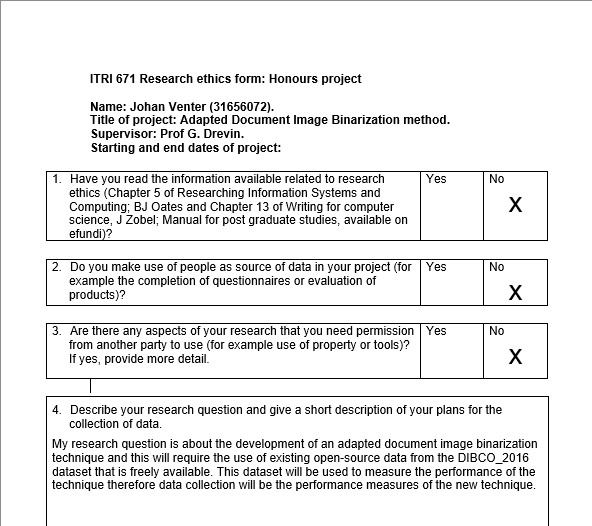
\includegraphics[width=\linewidth]{ethics1.png}
    \label{fig:ethics1}
\end{figure}
\begin{figure}
    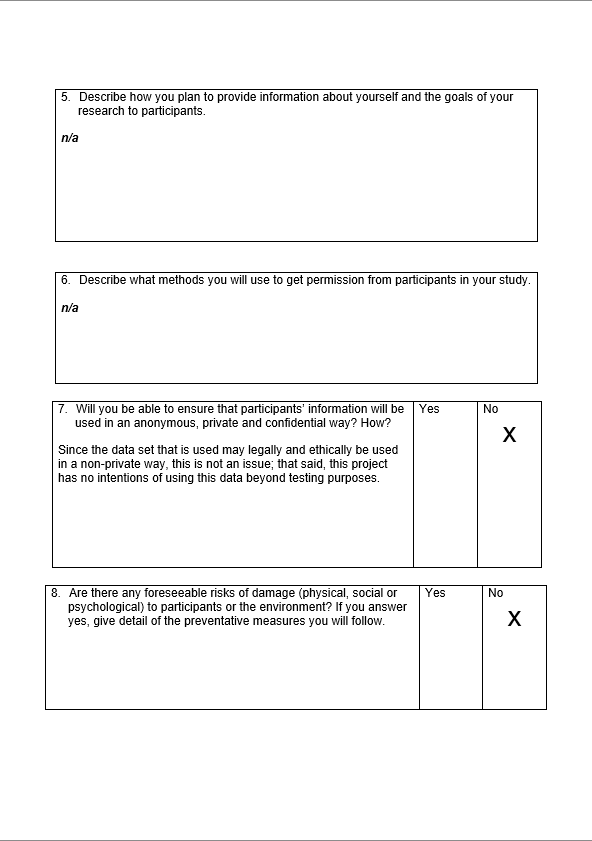
\includegraphics[width=\linewidth]{ethics2.png}
    \label{fig:ethics2}
\end{figure}
\begin{figure}
    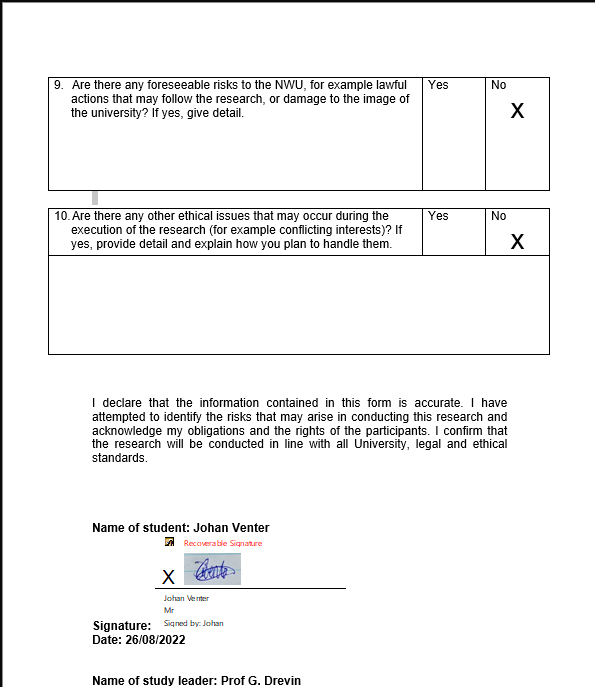
\includegraphics[width=\linewidth]{ethics3.png}
    \label{fig:ethics3}
\end{figure}

\section{Provisional Chapter Division}
\subsection{Introduction}
\subsubsection{Project Description}
\subsubsection{Problem Description and Background}
\subsubsection{Aims and Objectives of the Project}
\subsubsection{Procedures and Methods}
\subsubsection{Project Management and Plan}
\subsubsection{Development Platform, Resources and Environments}
\subsubsection{Ethical and Legal Implications and Dealing with These}
\subsubsection{Provisional Chapter Division}
\subsection{Literature Review}
\subsubsection{Image Processing Pipeline}
\subsubsection{Document Image Degradation}
\subsubsection{Issues With Modelling}
\subsubsection{Modelling}
\subsubsection{Implementation}
\subsubsection{Conclusion and Closing Remarks}
\subsection{Development of the Artefact}
\subsubsection{Description of the Artefact}
\subsubsection{Development Lifecycle}
\subsubsection{Development of the Artefact}
\subsection{Results}
\subsection{Reflection}
\subsection{Bibliography}

\chapter{Literature Review}
This chapter will discuss the ideas and challenges surrounding the binarization
of degraded document images. After discussing the image processing pipeline,
the first subsection discusses what degradation is, what its causes are, how
modelling is approached and lastly presents some current models.

\section{Image Processing Pipeline}
Image binarization falls into the pre-processing stage where degradation and
defects are compensated for. The pre-processing stage forms a pipeline of
processes that each modify its input before passing it to the next process in
the pipeline. The first of these is called the pre-processing stage where
degradation and defects are compensated for~\cite{ramanath2005color}. Since
this project is concerned with document images, the binarization of the
document also falls into the pre-processing stage.\par

Since document image binarization aims to separate the textual content from the
background by removing degradations, the first question arises: What does
degradation on an image look like and how does one model it?

\section{Document Image Degradation}
Degradations or defects on a document image refer to any properties of actual
document images that deviate from what can be considered the ideal image that
reduces the efficiency of image processing systems~\cite{Baird2007}. When paper
documents are printed, copied, faxed and scanned, the documents degrade. Even
if it seems insignificant to the human eye, this quality loss can reduce the
accuracy of even the most cutting-edge text recognition systems (OCR).
Additionally, there is mounting evidence that the quantity and
representativeness of training sets as well as the feature selection have a
considerable impact on the accuracy of stubborn picture pattern recognition
tasks~\cite{Baird2007}. Therefore, the performance of these algorithms hinges
on the quality of the binarization result. \par

\subsection{Operational Degradation}
This type of degradation involves the defects produced by the equipment used in
obtaining a digital copy of a given document image. An image is converted to
digital form using a scanning device. Unavoidable procedures result in the
introduction of a wide variety of noise and artefacts into the digital
document. Other noise patterns persist, such as the small imperfections in the
sensor's movements and architecture. Some corrections are automatically made by
the scanning devices. These corrections are mostly colour corrections, such as
"gamma correction," which adapts the scanned image to be displayed accurately
on a monitor~\cite{smoaca2011id}. Examples include the scanning of an image
that produces reflection artefacts or discrepancies due to an uncalibrated
sensor. The quality of the sensor will also affect the resolution of the
digital result. Since this type of degradation is caused by the scanner, it
tends to be easier to model since it is independent of the image and by
analysing the effects of the scanner on different images, one can model the
defects of the scanner.\par

An image is compressed into an image format like JPEG after it has been
scanned. Since this is a lossy compression standard, a significant portion of
the original image data is lost or altered~\cite{eskenazi2016stability}. \par

\subsection{External Degradation}
The physical deterioration of the original document is the main problem in this
situation. Examples of this type of degradation include blur, fluctuating
contrast, smudges and blotches, bleed-through text, variable character
intensities and stroke widths, artefacts that cover entire areas of text,
non-uniform noise or illumination, etc.~\cite{gatos2006adaptive}
~\cite{ait2022innovative}. This type of degradation refers to the defects
related to the physical state of the document, independent from the result
produced by the apparatus used to scan the document. This category of
degradation can be the most difficult to model as it cannot be generalized
since different degradations can appear at different intensities at various
locations in the document image. This can be further illustrated by the fact
that these types of degradation sometimes overlap with what is not considered
degradation. As an example, a model that may be good at identifying and
removing ink-smearing may compromise the quality of the document in areas where
ink-smearing is not present.

\subsection{Inevitable Disparities}
This type of degradation is described by the inevitable physical properties of
light, reflection, and the way that scanning devices scan images as well as
properties like the resolution of the images. Some of these degradations must
be modelled and analysed statistically~\cite{Baird2007}, but for some defects,
there are no existing models and are considered roadblocks in the image
pre-processing pipeline.

\section{Issues With Modelling}
~\cite{Baird2007} notes that the main components affecting the modelling process are:
\begin{itemize}
    \item \textbf{Parameterization}: The observed degradation must be able to be described by a fixed set of numerical parameters. Otherwise, the model is of no use.
    \item \textbf{Randomization}: If the degradation is modelled as having properties that behave in a probabilistic manner, their distributions should be parameterized in the model.
    \item \textbf{Validation}: Since some of the model parameters will inevitably be probabilistic, one needs to compensate for this by accounting for certain margins of error.
    \item \textbf{Parameter Estimation}: Once the model is developed, a distribution fitting the real distribution can be generated by tuning the parameters.
    \item \textbf{Correlation}: When modelling using statistics and probability distributions, one can easily mistake correlation for causation, therefore the model must be thoroughly evaluated by predicting the output of changes in parameters and verifying those predictions. Unexpected results may indicate that the model is incomplete.
\end{itemize}

\section{Modelling}
Document image degradation can be modelled in two main ways. The first is to
analyse and model the physical properties of the factors that cause these
defects. This can in turn deliver a degradation model based on the workings of
the environment that the images are subjected to. Although this method will
theoretically yield the most accurate, reliable results, this approach can
quickly become overcomplicated as~\cite{Baird2007} points out. The second
approach is to model the degradation empirically. This involves developing a
model that can replicate the effects of the degradation, disregarding the
cause. The main way this is done is by using statistical analysis. Of course,
these methods can be combined to form a hybrid model.

\subsection{Noise}
Image noise, which is typically introduced by electrical noise, is the random
variation in brightness or colour information in images. It can be created
using a scanner or a digital camera's image sensor and circuitry. This unwanted
by-product of image capturing known as image noise obscures desired
information. The devices used to scan documents introduce various forms of
noise to the document. Due to the random nature of noise, it is typically
modelled statistically. Since this topic has been the subject of research for a
significant amount of time (more than 80 years), existing noise models are very
sophisticated and although most models are statistics based, the papers also
consider the underlying physical structure of the scanning device in their
models such as the scanner model depicted by~\cite{gou2007robust} or the range
of noise patterns by imaging sensors modelled by~\cite{lukas2006digital}.\par

The following subsections describe common statistical methods used for noise
modelling.

\subsubsection{Gaussian Noise}
The most common type of noise found in images is Gaussian noise. It is an
additive noise model. The probability density function \(p\) of a Gaussian
random variable \(z\) is given by
\[p_{G}(z)=\frac {1}{\sigma {\sqrt {2\pi }}}e^{-{\frac {(z-\mu )^{2}}{2\sigma ^{2}}}}\]

where \(z\) is the pixel intensity, \(\mu\) the mean pixel intensity and
\(\sigma\) its standard deviation.

\begin{figure}[ht]
    \centering
    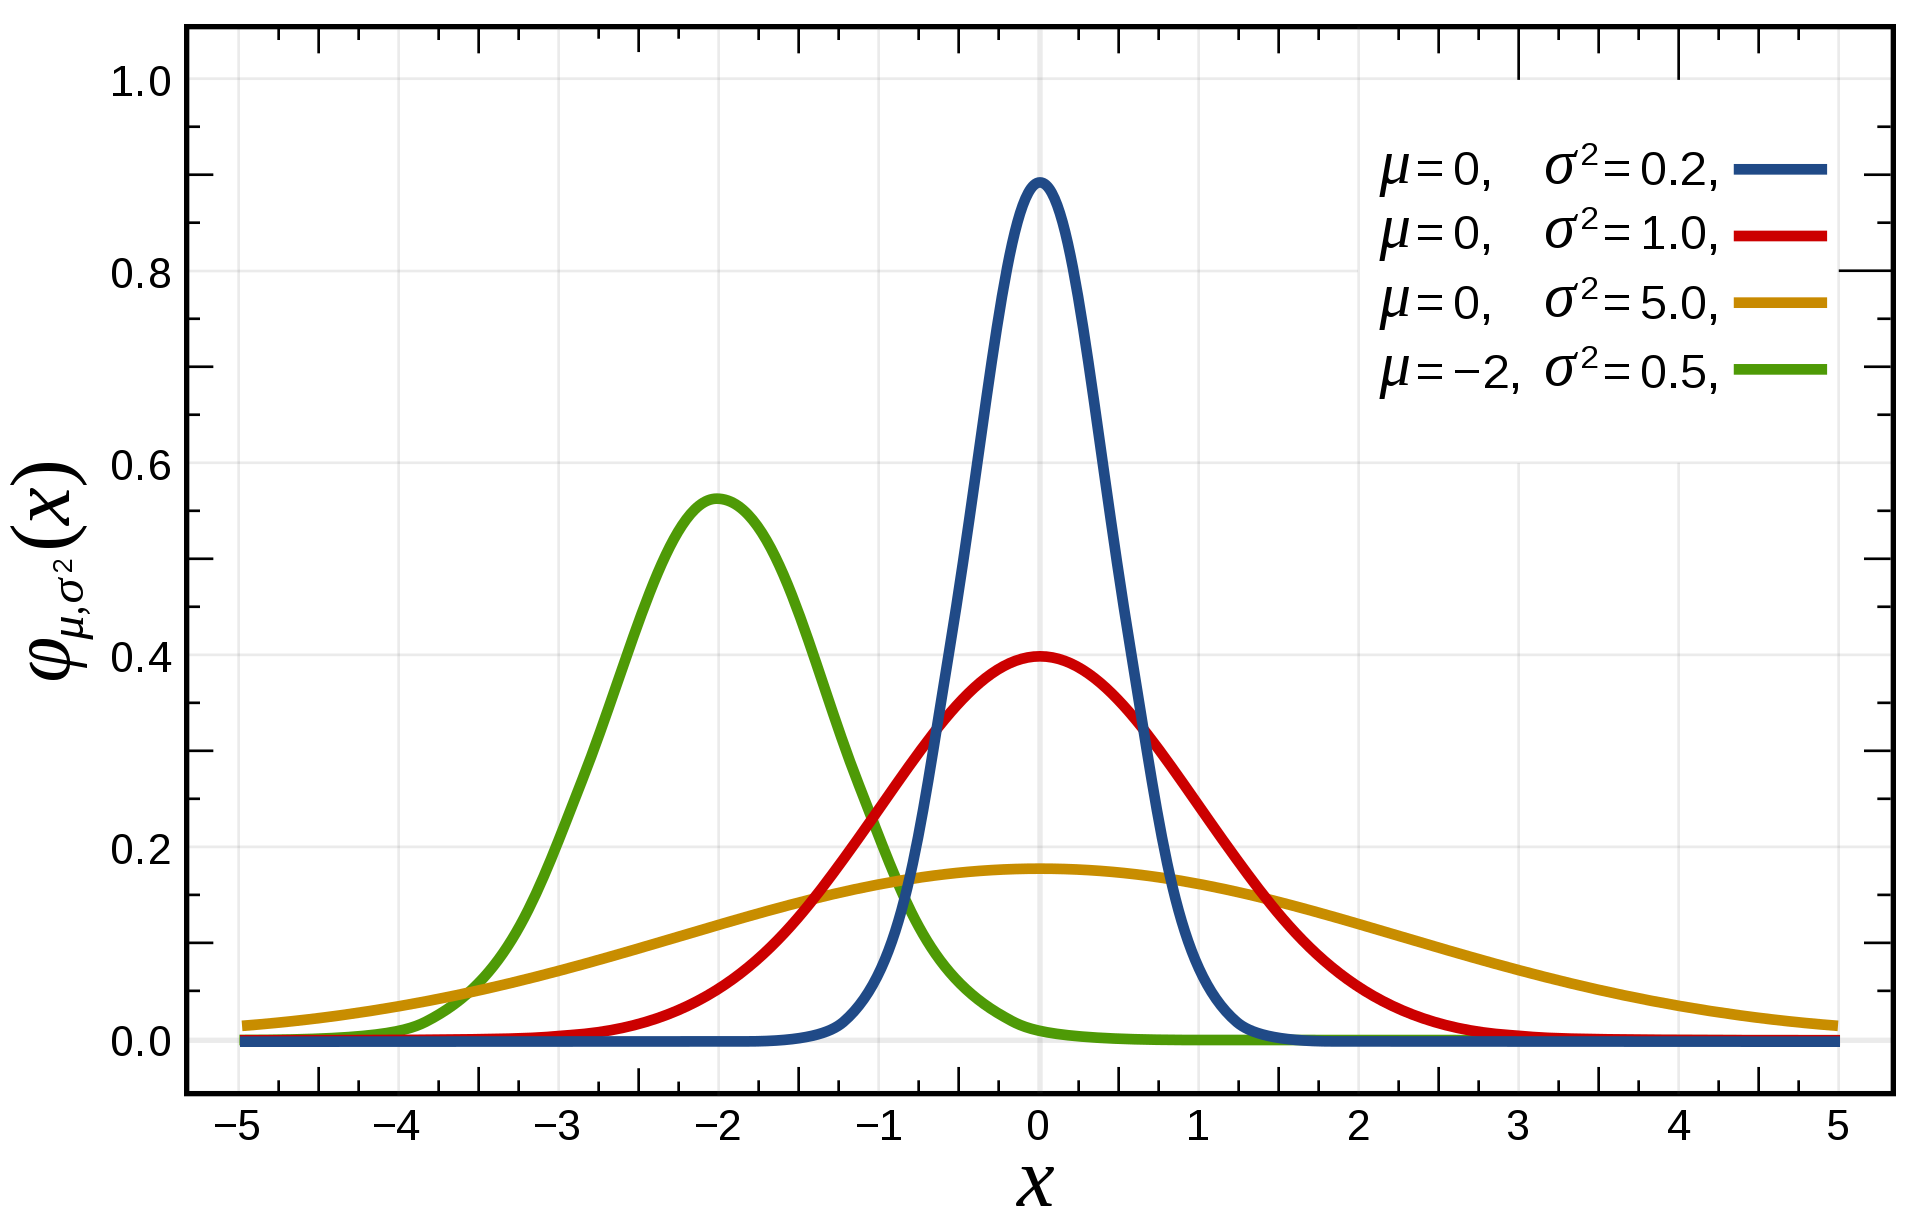
\includegraphics[width=8cm]{gaussian distribution.png}
    \caption{Gaussian PDF with different parameters~\cite{gaussian_image}}
    \label{fig:gaussian_image}
\end{figure}

\subsubsection{Impulse Noise (Salt and Pepper Noise)}
Impulse noise is characterised by sharp and rapid changes in the image signal.
It appears as sparsely distributed white and black pixels.

\subsubsection{Shot Noise}
Shot noise or Poisson noise occurs due to the statistical character of
electromagnetic waves and the random fluctuation of
photons~\cite{boyat2015review} and is modelled by the Poisson distribution. The
Poisson distribution is a function of a discrete random variable X.
\[P(k)=\frac{\lambda^{k}e^{-\lambda}}{k!}\]
with \(\lambda > 0\)
\begin{figure}[ht]
    \centering
    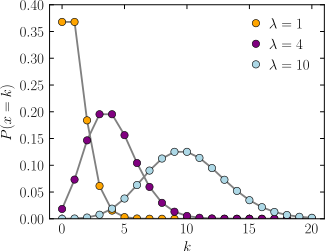
\includegraphics[width=8cm]{poisson distribution.png}
    \caption{Poisson PDF with different parameters~\cite{poisson_image}}
    \label{fig:poisson_image}
\end{figure}

Other noise models include Rayleigh noise, Gamma noise, Exponential noise and
Uniform noise each having a probability density function that describes the
distribution of the noise in an image~\cite{gonzalez_woods_pearson_hall}.\par

Noise can be classified according to which domain it is filtered in. Noise
removal can either be done in the spatial domain or the frequency domain.
Images must undergo the Fourier Transform to map them onto the frequency
domain. In spatial domain filtering there exist some popular methods such as
Mean, Wiener and median filtering. Filtering in the frequency domain yields
many more opportunities such as filtering in the wavelet domain using linear,
non-linear, and other models.

\subsection{Scanner Degradation Model}

An image is scanned by a scanning device using a light-sensitive sensor. This
sensor senses the light reflected by the document in some neighbourhood of a
pixel in the image close to the sensor. Since the surrounding areas affect the
signal received by the sensor, some distortion is introduced that can be
modelled. This type of distortion is typically modelled as a Point Spread
Function (PSF).~\cite{smith1998characterization} provides a method for
estimating a point spread parameter \(\delta_c\) that is dependent on the
period of a detected pulse \(\tau\), the width of a square pulse \(\omega\) and
some pre-decided thresholding value \(\Theta\), delivering a piecewise
function:
\[
    \delta(\tau)=
    \begin{cases}
        \frac{\tau}{2}             & A \\
        \omega(\frac{1}{2}-\Theta) & B \\
        -\frac{\tau}{2}            & C \\
    \end{cases}
\]
A, B and C represent sections of the scanned image with decreasing density
(number of black pixel sections and white pixel sections per area). This model
is used to generate synthetic characters that mimic the point spread in the
signal received by a scanner and is implemented in the training models of
classifier systems as well as evaluation benchmarks for OCR.

\begin{figure}[ht]
    \centering
    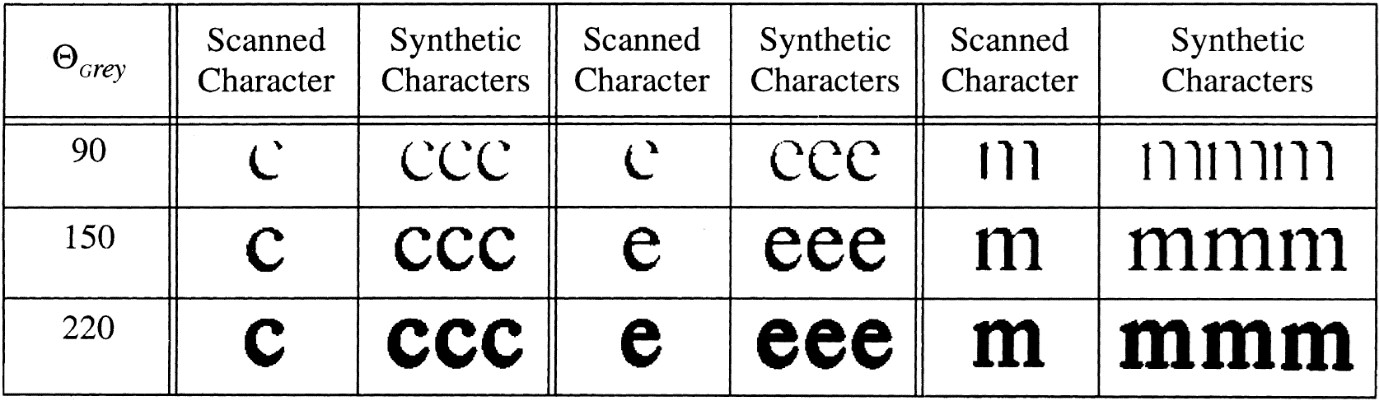
\includegraphics[width=8cm]{scanner.jpg}
    \caption{Synthetic Characters~\cite{smith1998characterization}}
    \label{fig:scanner}
\end{figure}

\subsection{Character Degradation Modelling}
The most common type of degradation is some sort of distortion of the
characters of the document. These common types include ink blotches and smears.
This type of degradation is characterised by dark areas over or around a
character. The paper by~\cite{kieu2012character} proposes a method that models
this as a region of noise, They use a formula that describes a region of noise
as an elliptic area wherein a random generation function following the normal
distribution \(N(\mu,\sigma x^2)\) is used to generate noise where \(\sigma\)
is an input parameter and \(\mu\) is calculated based on pixel values in the
segment where the noise will be added.

The results of their model by varying the \(\sigma\) parameter:

\begin{figure}[ht]
    \centering
    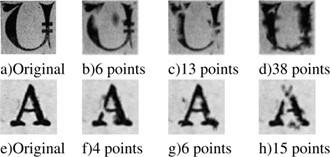
\includegraphics[width=8cm]{char_degradation.jpg}
    \caption{Varying the \(\sigma\) parameter~\cite{kieu2012character}}
    \label{fig:char_degradation}
\end{figure}

This model sufficiently mimics the defects present in documents affected by
natural elements. In the paper, they note that the performance of OCR goes down
as the number of defects increases, and as such these artificial characters are
also used for training classifier systems.

\section{Implementation}

\subsection{Noise Removal}
The first step in document binarization is to remove the various forms of noise
present in the images. The method used is dependent on the characteristics of
the noise identified as using the wrong model will not remove the noise
effectively and compromise the quality of the image.

\subsubsection{Median Filter}
The median filter traverses the pixels of the image and replaces the values of
the pixels with the median value in some neighbourhood around the pixel called
a window. The grey values inside the window are ordered and the centre pixel’s
value is replaced with the median grey value. This technique is nonlinear and
highly effective at removing salt-and-pepper noise since sudden jumps in grey
value magnitudes are removed. The median filter is however not very
computationally efficient since sorting takes a lot of time.

\subsubsection{Wiener Filter}
Wiener filtering is a popular statistical noise removal method based on
minimising the mean square error for stationary Gaussian
process~\cite{jin2003adaptive}. By this measure, the wiener filter is the
optimal filter. The basic model is directed towards finding an estimator
\(\hat{x}\) for the original image S that minimises:
\[MSE(\hat{x})=\frac{1}{N} \sum_{i,j\in S}^{N}(\hat{x}(i,j)-x(i,j))^2\]
They can be treated as stationary since Gaussian noise is considered globally
independent noise. The filter takes two parameters \(\mu\) being the signal
mean and \(\sigma^2\) the signal variance. While the global version uses global
statistics of the image to minimise the error, the local version is more
adaptive and calculates the statistics in different neighbourhoods in the
image.
\par

~\cite{gatos2006adaptive} describes the use of an adaptive wiener filter that makes use of the local properties in an image to reduce noise using the following formula:
\[I(x,y)=\mu+\frac{(\sigma^2-v^2)(I_{source}-\mu)}{\sigma^2}\]
where \(\mu\) is the local mean, \(\sigma^2\) the variance in a 3 x 3 window
and \(v^2\) is the average variance.
\par
The Wiener-Hunt filter is a variation on the original Wiener filter, that
transforms the image into the frequency domain first by using the Fourier
transform
\[\hat x = F^\dagger (|\Lambda_H|^2 + \lambda |\Lambda_D|^2)
    \Lambda_H^\dagger F y\]
with \(F\) and \(F^\dagger\) the Fourier and inverse Fourier transforms
respectively, \(\Lambda_H\) the Fourier transform of the transfer function and
\(\lambda\) a damping constant as described by~\cite{scikit-image}.

\subsubsection{Wavelet Filter}
The wavelet transform decomposes the image into a collection of wavelets. A
wavelet is a wave-like function, that has a finite 'energy' and a symmetric
area around the x-axis. The transform can be interpreted as the convolution of
a set of wavelets over the image that will output a signal proportional to the
similarity between the wavelets and the image.\par

Similar to the Fast Fourier Transform (FFT), a Wavelet transform separates
image intensities into frequency components. These components are modified and
then transformed back to the spatial domain. The wavelet extends across a
finite distance, which gives it an advantage over Fourier
approaches~\cite{wavelet_filtering_2022}.
\[ \int_{-\infty}^{\infty} f(x,y) \cdot g(x,y) \,dx \]

\subsubsection{Kuan Filter}
By substituting the core pixel with a weighted average of the centre pixel and
the mean of the values in a square kernel surrounding the pixel, the Radar Kuan
filter determines the value for each pixel. Edge pixel values are duplicated to
create enough data to filter pixels close to the image's edges.

The main purpose of this filter is to reduce speckle noise. While reducing the
loss of radiometric and textural information, it smooths image data without
eliminating edges or sharp features in the images. The multiplicative noise
model is initially changed by the Kuan filter into a signal-dependent additive
noise model. The model is then subjected to the least mean square error
criteria~\cite{kuan_filter_2022}. The smoothed pixel's calculated grey-level
value (R) is:
\[R=xW+\mu(1-W)\]
where
\begin{itemize}
    \item \(x\) is the centre pixel in a neighbourhood
    \item \(\sigma\)= standard deviation of pixel intensities in the window
    \item \(\mu\)= mean of the pixel intensities in the window
    \item \(i=\frac{\sigma}{\mu}\)
    \item \(u=\sqrt{\frac{1}{number of iterations}}\)
    \item \(W=\frac{1-\frac{u^2}{i^2}}{1+u^2}\)
\end{itemize}
~\cite{kuan_filter_2022}\par

Other Denoising methods were considered such as total-variation denoising and
bilateral denoising.

\subsection{Edge Detection}
Edge detection is a technique in image processing that highlights the
boundaries of objects in images by identifying areas with high contrast.

\subsubsection{Variance Edge Detection}
By calculating the variance of the intensities of pixels in a neighbourhood,
one can construct a simple basic edge detector:
\[S^2=\frac{\sum^N{(x_i-\bar{x})^2}}{N-1}\]
with $N$ being a dimension of the image

\subsubsection{Canny Edge Detection}
The Canny edge detection algorithm works as follows:
\begin{enumerate}
    \item A Gaussian filter is convolved to remove noise.
    \item The intensity gradient of the image is calculated by using directional edge
          operators such as Roberts, Prewitt or Sobel.
    \item The gradient magnitude is calculated and used as an upper and lower threshold
    \item Track edges by hysteresis.
\end{enumerate}

~\cite{rong2014improved} outlines the principal part of the algorithm where the edges are identified by calculating the gradient between pixels. The following first-order partial derivative estimations are used on the original image \(I\) for pixels \(i,j \in I\):

\[E_x(i,j)=\frac{1}{2}(I(i+1,j)-I(i,j)+I(i+1,j+1)-I(i,j+1))\]
\[E_y(i,j)=\frac{1}{2}(I(i,j+1)-I(i,j)+I(i+1,j+1)-I(i+1,j))\]
which can also be written in matrix form as
\[\mathbf{G}_x=\begin{bmatrix}
        -1 & 1 \\
        -1 & 1 \\
    \end{bmatrix},
    \mathbf{G}_y=\begin{bmatrix}
        1  & 1  \\
        -1 & -1 \\
    \end{bmatrix}
\]

The magnitude is calculated as
\[|\mathbf{G}|=\sqrt{\mathbf{G}_x^2+\mathbf{G}_y^2}\]
and the edge direction as
\[\Theta=atan2(\mathbf{G}_y,\mathbf{G}_x)\]

~\cite{rong2014improved}identifies some problems with the traditional Canny algorithm. The first is that since the convolution window is a 2x2 matrix, it is sensitive to noise. Seeing that the algorithm uses the partial derivatives in the x and y direction, it is not sensitive to edges oriented $90^{\circ}$ relative to the major axes.\par

Due to this, some augmented methods have been constructed that attempt to solve
these issues such as those proposed by~\cite{rong2014improved}
and~\cite{xuan2017improved}

\subsubsection{Contrast Edge Detection}
An image is constructed using a formula for identifying local image contrast as
proposed by~\cite{su2012robust}.
\begin{equation}
    \label{E:1}
    C(i,j)=\frac{I_{max}(i,j)-I_{min}(i,j)}{I_{max}(i,j)+I_{min}(i,j)+\epsilon}
\end{equation}
where \(\epsilon\) is a positive infinitesimal. The denominator scales the input according to the local range of values, thereby normalizing the contrast across the image~\cite{su2012robust}. Next, a constant \(a\) is calculated:
\begin{equation}
    \label{E:2}
    a=(\frac{\sigma}{128})^\gamma, \; \gamma \geq 0
\end{equation}
\(\sigma\) is the standard deviation of the entire document image intensities.
By combining \ref{E:1} and \ref{E:2} we derive the final equation they use to construct the Gradient image:
\begin{equation}
    \label{E:3}
    C_a(i,j)=a\times C(i,j)+(1-a)(I_{max}(i,j)-I_{min}(i,j))
\end{equation}

\subsection{Thresholding}
Thresholding is the technique of converting a grayscale image to black and
white by turning just the pixels whose values are higher than a specified
threshold into white and the other pixels into black~\cite{inproceedings}. A
straightforward method of segmenting images is image thresholding. This is
frequently done to segregate "object" or foreground pixels from background
pixels by designating pixel intensities one of two values depending on a
comparison with a calculated threshold value.

\subsubsection{Binary Thresholding}
A binary threshold will set all values larger than a calculated threshold value
to 1 and all other values to 0.
\[
    i(x,y)=
    \begin{cases}
        1 & I(x,y) > T    \\
        0 & I(x,y) \leq T
    \end{cases}
\]
with threshold value $T$

\subsubsection{Niblack's Method}
The Niblack local thresholding method calculates a threshold $T$ in every
neighbourhood around every pixel in the image~\cite{scikit-image}.
\[T=\mu-k*\sigma\]
where a chosen $k$ scales the standard deviation parameter $\sigma$

\subsubsection{Sauvola's Method}
The Sauvola local thresholding method calculates a threshold $T$ in every
neighbourhood around every pixel in the image~\cite{scikit-image}. This method
is an adaptation of Niblack's method.
\[T=\mu*\frac{R+k*(\sigma-R)}{R}\]
where a chosen $k$ scales the standard deviation parameter $\sigma$

\subsubsection{Otsu's Method}
Otsu's method is an automatic image thresholding approach. The algorithm
returns a single intensity threshold, dividing pixels into the foreground and
background classes. This threshold is calculated by optimising for inter-class
and intra-class variance. The algorithm uses an exhaustive search for the
threshold parameter that minimises the intra-class variance defined as:
\[\sigma_{\omega}^{2}(t)=\omega_0(t)\sigma_0^2(t)+\omega_1(t)\sigma_1^2(t)\]
with $\omega_0$ and $\omega_1$ the probabilities and $\sigma_0^2$ and
$\sigma_1^2$ the variances of the mutually exclusive classes. The threshold is
then selected as the maximum value of $\sigma_{\omega}^{2}$.
\begin{figure}[ht]
    \centering
    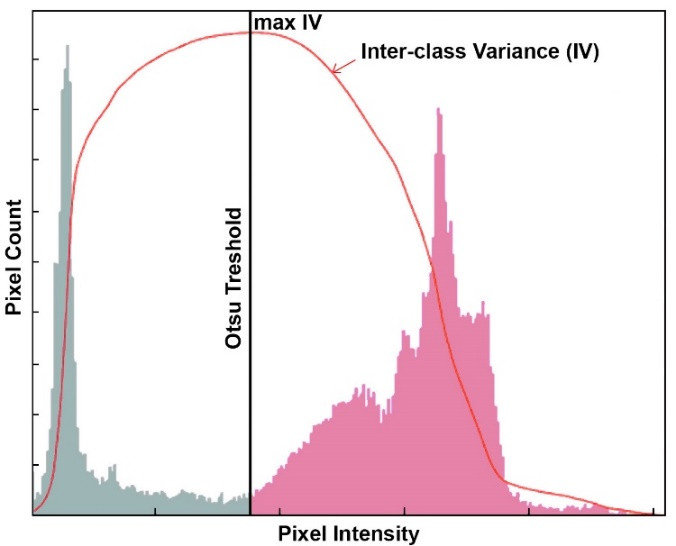
\includegraphics[width=8cm]{otsu.png}
    \caption{Otsu Visualization~\cite{mdpi_2020}}
    \label{fig:otsu}
\end{figure}

\subsection{Other Useful Concepts}
\subsubsection{Distance Transform}
The distance transform is applied to a binary image. It then assigns a value to
every foreground pixel using some distance measure. Although many different
distance measures (briefly illustrated in Figure \ref{fig:distances}) exist,
the most used measures are the chessboard or euclidean distance measures.
\begin{figure}[ht]
    \centering
    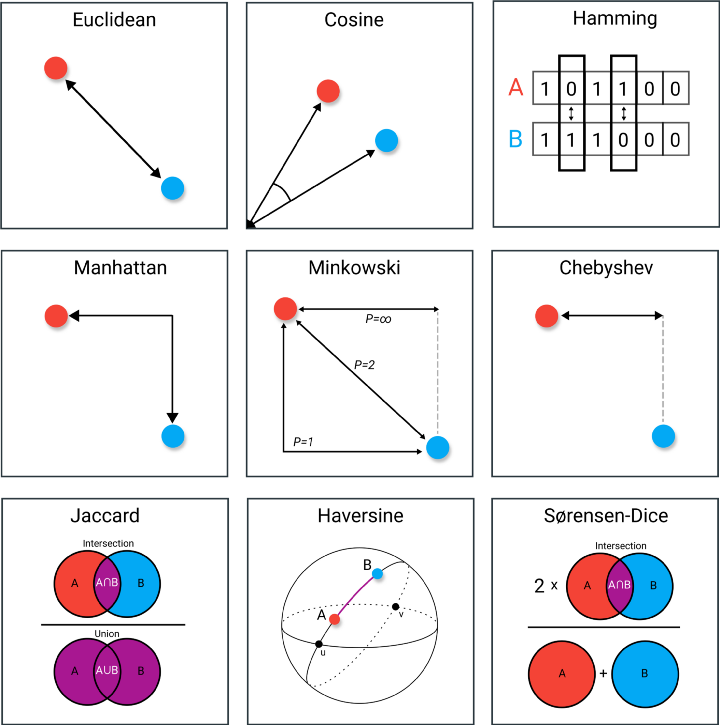
\includegraphics[width=8cm]{distances.png}
    \caption{Distance Measures~\cite{distance_measures}}
    \label{fig:distances}
\end{figure}

\begin{figure}[ht]
    \centering
    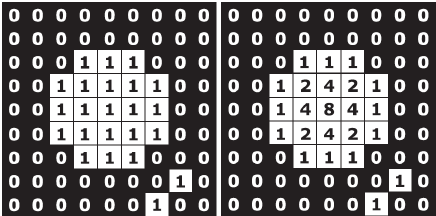
\includegraphics[width=8cm]{distance_transform.png}
    \caption{Distance Transform(Squared Euclidean)~\cite{distance_transform}}
    \label{fig:dt}
\end{figure}
Each foreground pixel intensity is assigned the value of its distance to the closest background pixel.
\begin{itemize}
    \item \textbf{Euclidean}: $i(x,y)=\sqrt{bg(x,y)^2+fg(x,y)^2}$
    \item \textbf{Chessboard}: $i(x,y)=|bg(x,y)|+|fg(x,y)|$
\end{itemize}

\subsection{Post Processing}
After the image has been binarized it can finally be used in OCR programs and
other sorts of post-processing endeavours such as stroke analysis and other
typographic analysis meant to discover patterns and tendencies in written text
such as handwriting recognition and adaptive natural typeface generation.

\section{Conclusion and Closing Remarks}
This section has discussed a collection of popular techniques and methods used
in binarizing document images. A central idea is identified that gets expanded
upon in the different papers. All the techniques and models are based on the
identification of some pattern following the development of a function that
implements the model. This project will be testing and evaluating some of the
discussed methods as well as new ones should their relevance become apparent.
There are some existing libraries for use in the python programming language
that have an extensive collection of image processing-related functions. Should
any of the necessary functions be missing they will be implemented using their
theoretical models. After implementing these methods, their performance will be
evaluated and compared using the DIBCO 2016 document image dataset. This
dataset is comprised of 10 different document images along with 10 ideal images
that have no degradation.

\chapter{Development of the Artefact}

\section{Description of the Artefact}
The development of this artefact was inspired by the method used
by~\cite{su2012robust} for document image binarization. Document Image
Binarization, in this context, is a field of study within the phase of image
pre-processing where a digital version of a written document is transformed
into a binary image, separating the text from the noise, degradation and
background~\cite{su2012robust}. Therefore, this artefact had a clear objective,
namely, to obtain a digital written document, process the image by removing
unwanted artefacts and deliver a binary image containing only the text from the
original image.\par

This artefact, therefore, is a program written in python that receives a
document image as input and then passes the image through a pipeline of
distinct processes, each modifying the image or extracting information about
the image for use in the following process. The resulting program uses three
main libraries namely \href{https://numpy.org/}{numpy}~\cite{numpy},
\href{https://scikit-image.org/}{scikit-image}~\cite{scikit-image} and
\href{https://scikit-image.org/}{scipy}~\cite{2020SciPy-NMeth} in conjunction
with custom-developed methods to compose the processes that make up the
pipeline. \par

The process is comprised of four main steps. The images used for testing and
demonstrations are open-source, provided by
\href{https://vc.ee.duth.gr/h-dibco2016/}{DIBCO 2016 Handwritten
    DocumentDataset}.

\subsection{Conversion to Greyscale}
The testing dataset contains images with three colour channels as well as
single colour channel images. To cohere images for processing, each document
image is provided as input and is converted to a grayscale image. This is done
by averaging the three colour channels of the image into a single channel. The
images that are already greyscaled are left intact.

\[grey(x)=\frac{r(x)+g(x)+b(x)}{3}\]

\subsection{Normalizing}
The images are all greyscale, but their intensity values cover vastly different
ranges at different scales. Therefore, the next step is to normalize the
intensity values of the image $S$ by scaling them to fall into a range
$f:\mathbb{R} \mapsto [0,1]$ and
\[f(x)=\frac{x-min(S)}{max(S)-min(S)}\]
for each $x \in S$. This does not affect the way the image looks since the
\textit{\textbf{imsave}} function in the textit{\textbf{matplotlib}} library
automatically rescales the intensity values when the generated image is saved.

\begin{figure}[ht]
    \centering
    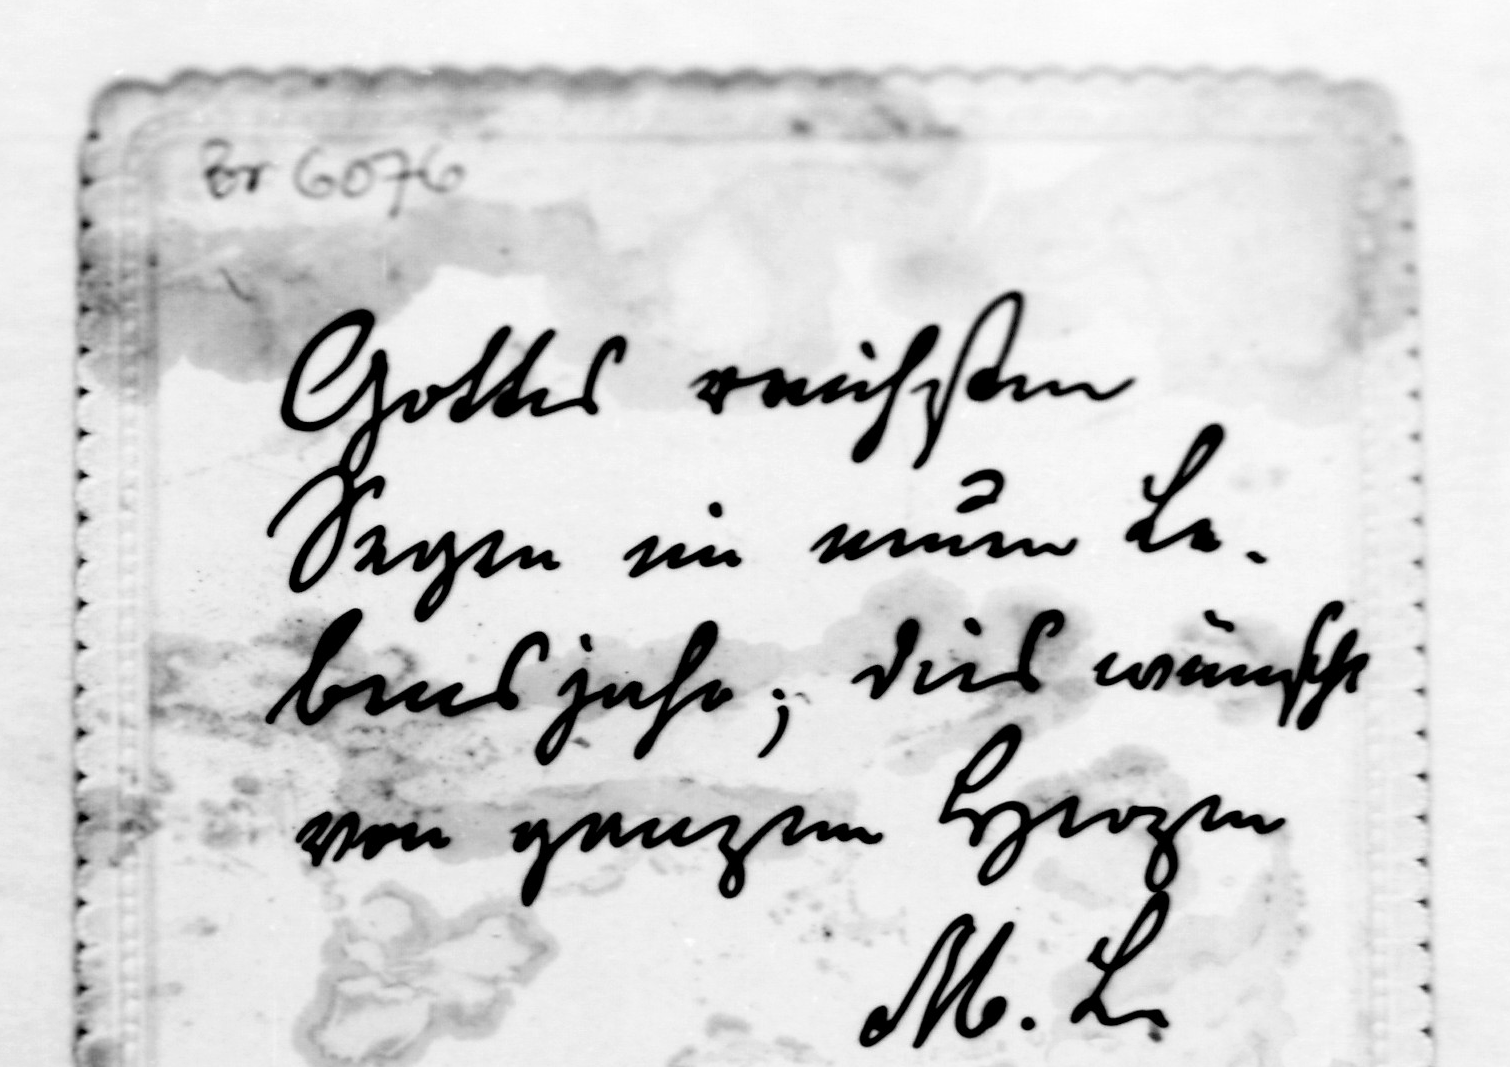
\includegraphics[width=6cm]{original.png}
    \caption{Original Document Image}
    \label{fig:1}
\end{figure}

\subsection{Denoising}
After the image is converted to grayscale and normalized, the image is
denoised. Both low and high-frequency noise is prevalent in most images. The
low-frequency noise or coarse noise is filtered by applying the wavelet
denoising filter available in the scikit-image library. This filter uses the
standard deviation of the intensity values of the image as an input parameter
as demonstrated in Figure~\ref{fig:2}.

\begin{figure}[ht]
    \centering
    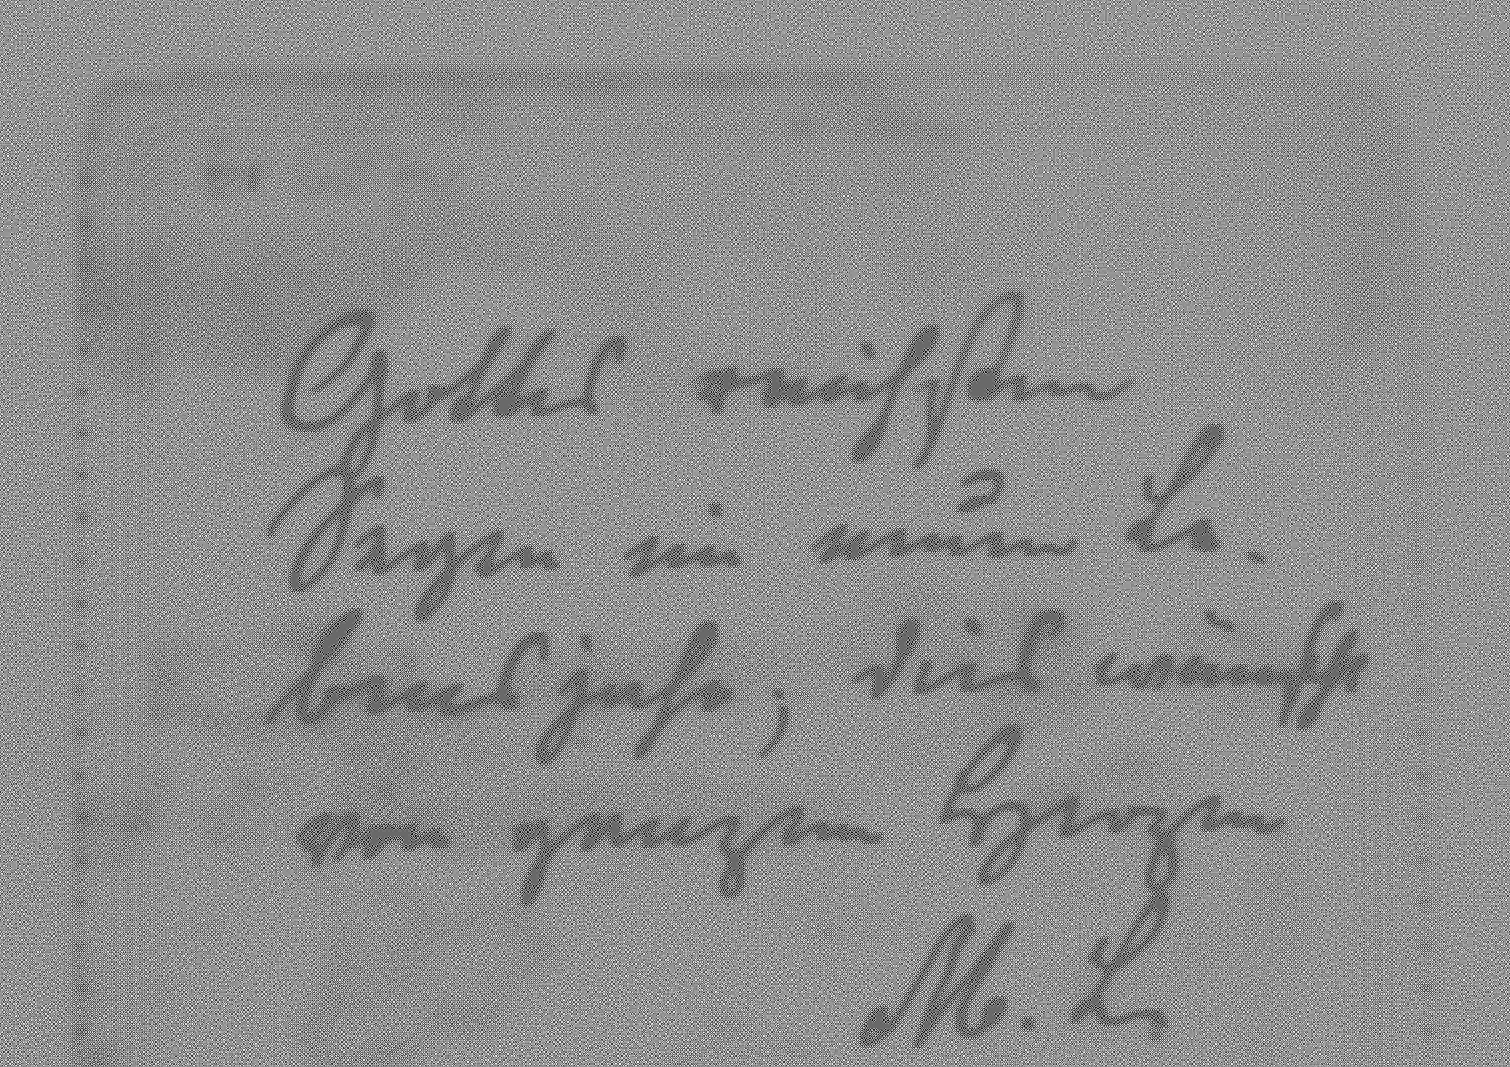
\includegraphics[width=6cm]{wavelet difference.png}
    \caption{Noise removed by wavelet filter}
    \label{fig:2}
\end{figure}

This is followed by applying a custom adaptive wiener filter that generates a
3x3 kernel with a centred gaussian distribution. The image undergoes the Fast
Fourier Transform (FFT) and then uses the gaussian kernel to convolve over the
image; removing low-frequency gaussian noise (Figure~\ref{fig:3}). Lastly, the
image is transformed back to the spatial domain. Note, at this point, that the
image's grey-level intensity values cover a vast range.

\begin{figure}[ht]
    \centering
    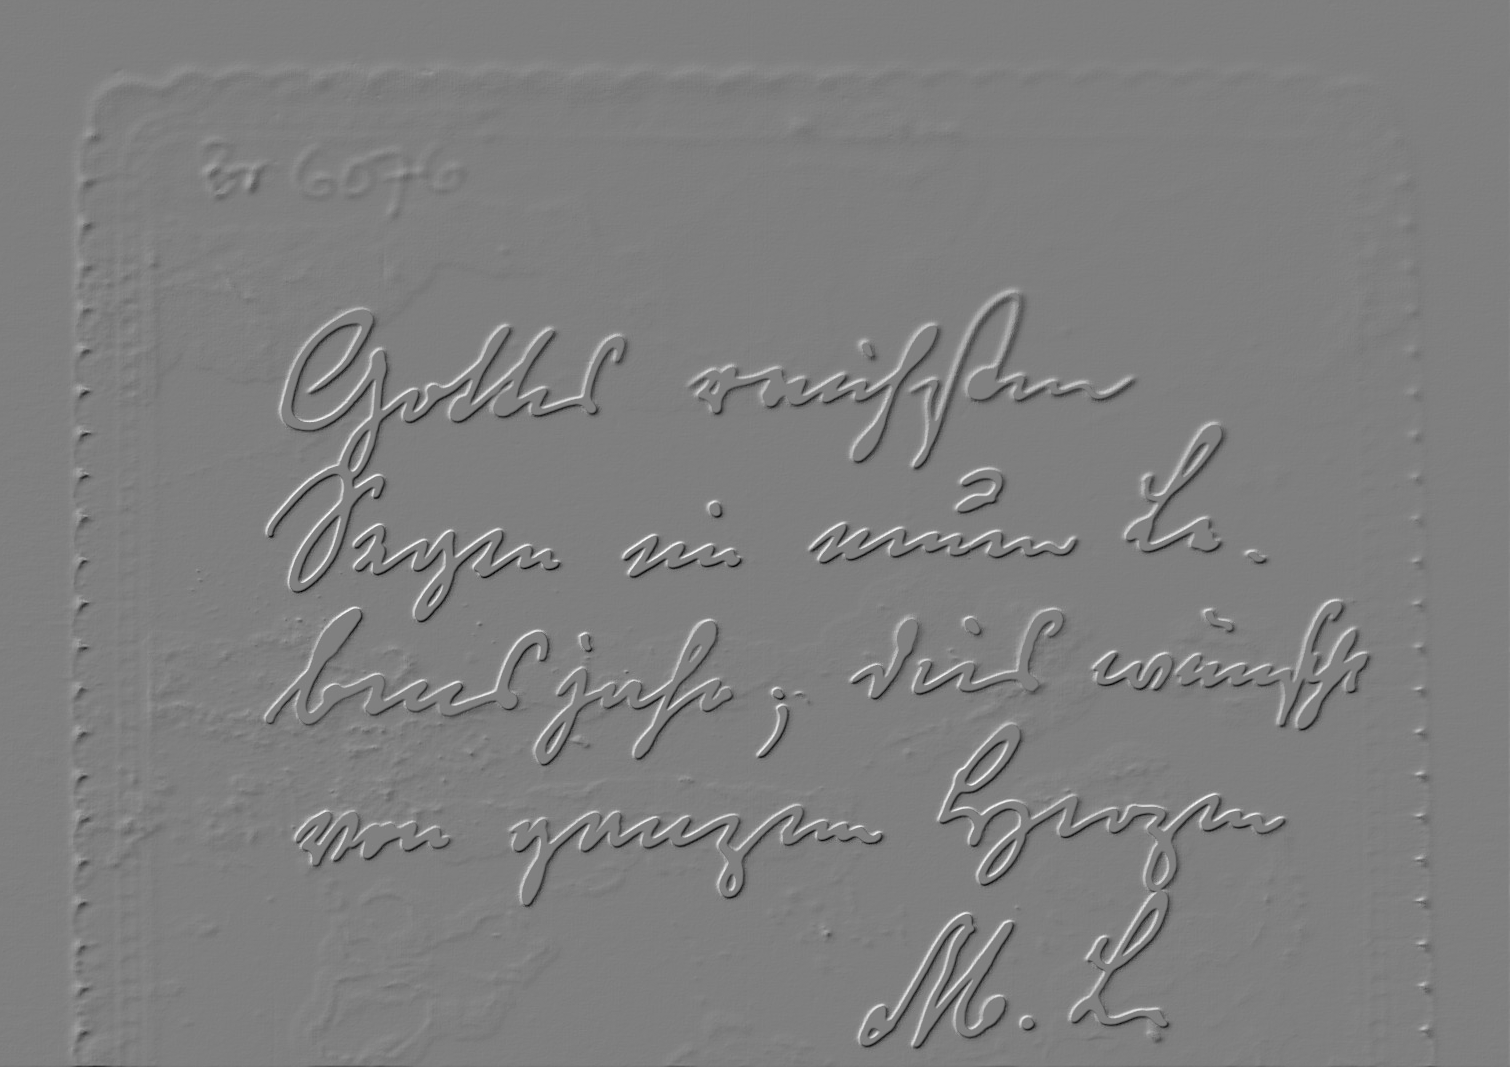
\includegraphics[width=6cm]{wiener difference.png}
    \caption{Noise removed by Wiener filter}
    \label{fig:3}
\end{figure}

\subsection{Thresholding}
Otsu's thresholding method is used to convert the denoised image into a binary
image.

\begin{figure}[ht]
    \centering
    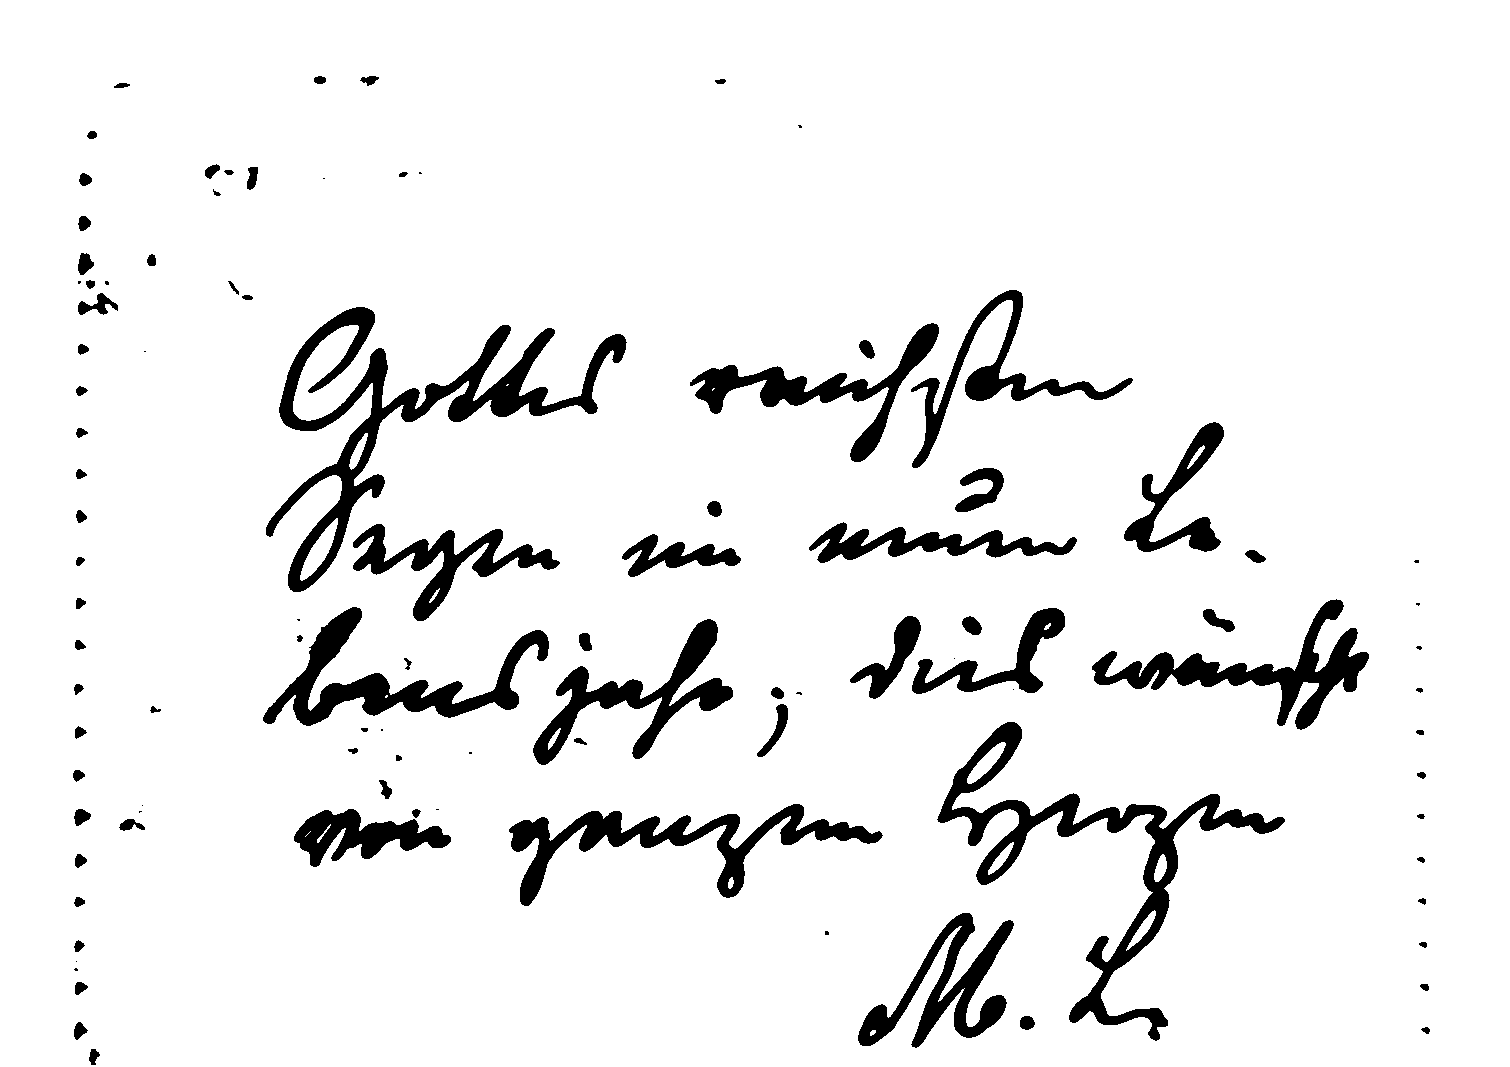
\includegraphics[width=6cm]{otsu thresholded.png}
    \caption{Otsu thresholded image}
    \label{fig:4}
\end{figure}

\subsection{Text Stroke Width Estimate}
An estimation of text stroke width will be utilised in the final step. An
effective method of doing this as introduced by~\cite{strokewidth} consists of
two main steps, namely performing a distance transform and then skeletonizing
the image.

\subsubsection{Distance Transform}
The distance transform uses the thresholded image and assigns each pixel a
value according to its euclidean distance to the closest white pixel
(background pixel), thereby creating an image with the brightest pixels in the
centre of the text.

\begin{figure}[ht]
    \centering
    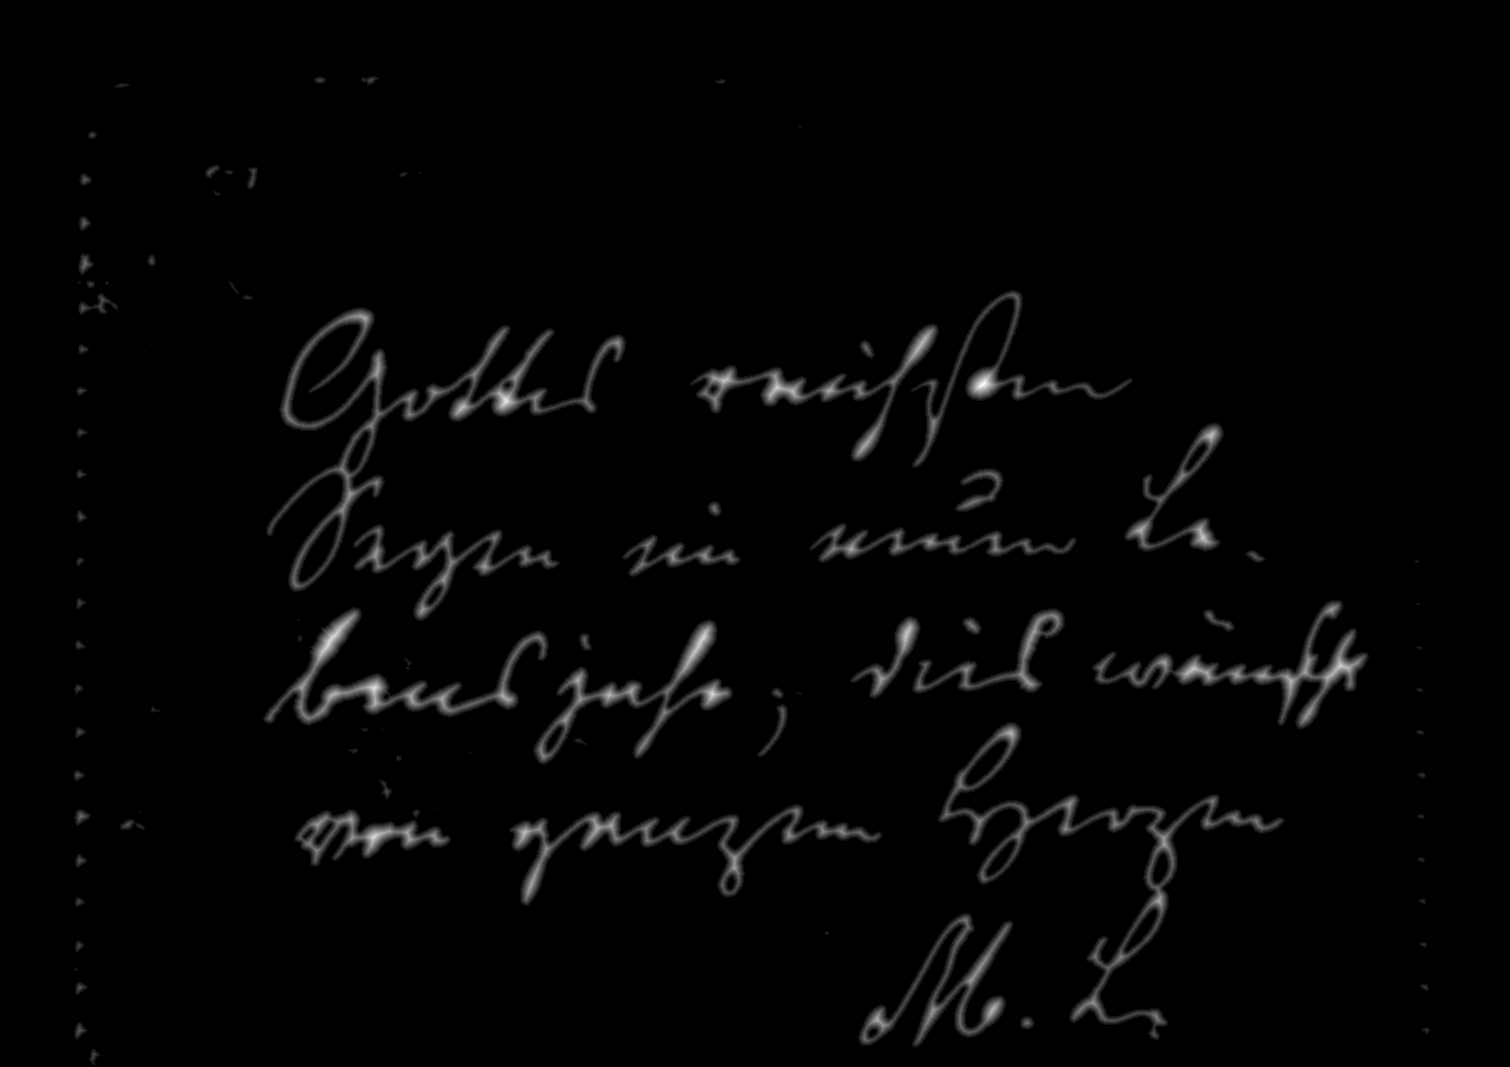
\includegraphics[width=6cm]{distance transform.png}
    \caption{Distance transform}
    \label{fig:5}
\end{figure}

\subsubsection{Skeletonizing}
Skeletonizing an image consists of making multiple passes over an image and
detecting the edge pixels. These edge pixels are then removed unless they break
the connectivity of the identified object~\cite{scikit-image}. The implemented
method is the Zhang adaptation~\cite{zhang_suen_1984} that traverses the image
and removes the boundary and corner points of foreground sections. Doing this
iteratively leaves only a 1-pixel-wide skeleton.

\begin{figure}[ht]
    \centering
    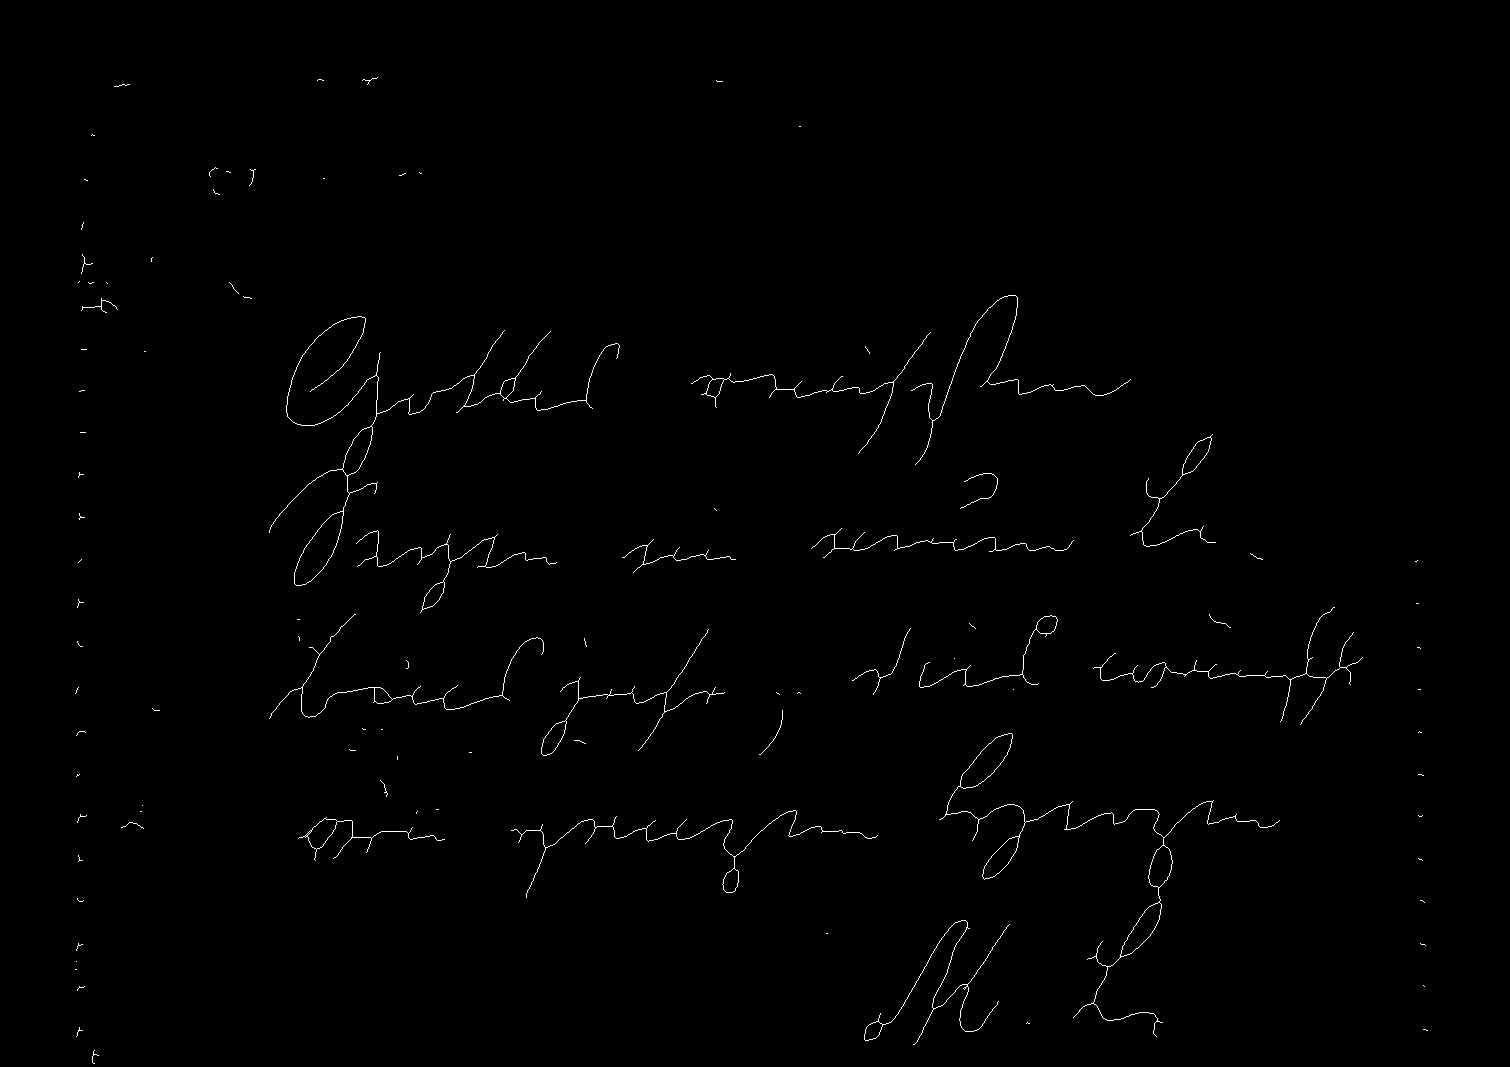
\includegraphics[width=6cm]{skeletonized.png}
    \caption{Skeletonizing transform}
    \label{fig:6}
\end{figure}

Since the pixels in the middle of each stroke are the furthest away from the
background pixels and the skeletonized image contains white pixels only in the
centres of the stroke, the indexes of the foreground (bright) pixels in the
skeletonized image are iterated in the distance-transformed image. The selected
pixel values in the distance-transformed image are summed and averaged to
obtain a quantity half of the actual average text stroke width since it
measured the distance from the centre of the stroke to the edge of the stroke,
therefore half of the actual width.

\subsection{Median Filter}
Finally, A median filter that uses the calculated stroke width as the window
size for convolution passes over the image to remove artefacts on the image
smaller than the text stroke to produce the final result.

\begin{figure}[ht]
    \centering
    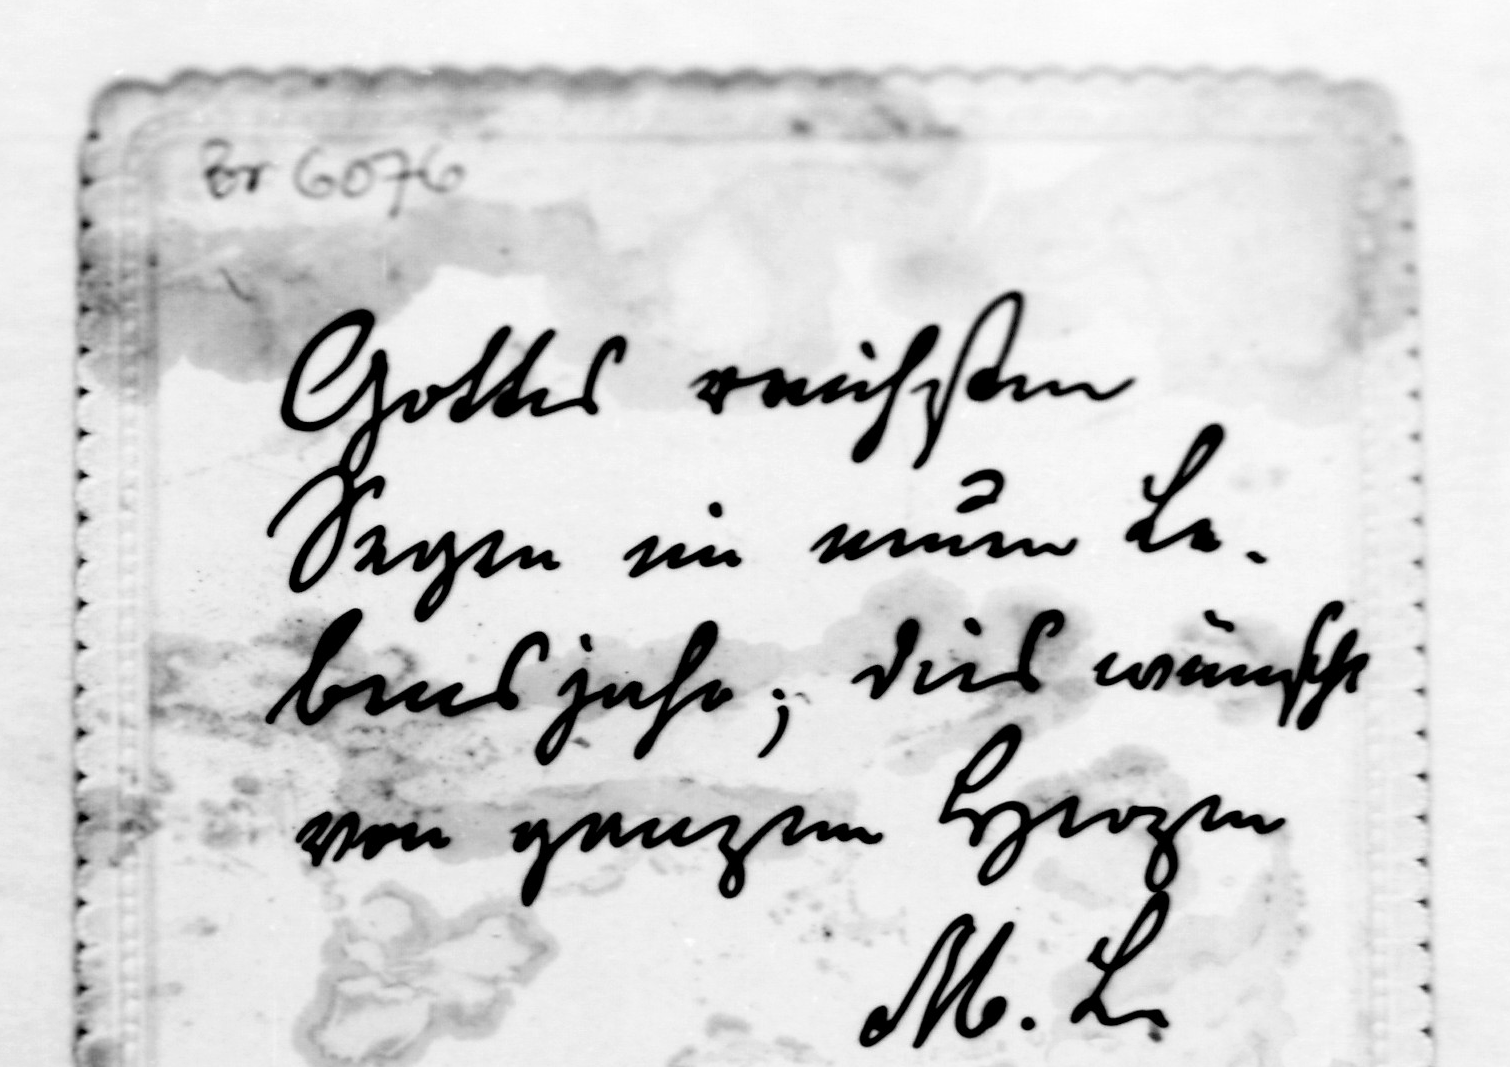
\includegraphics[width=8cm]{original.png}
    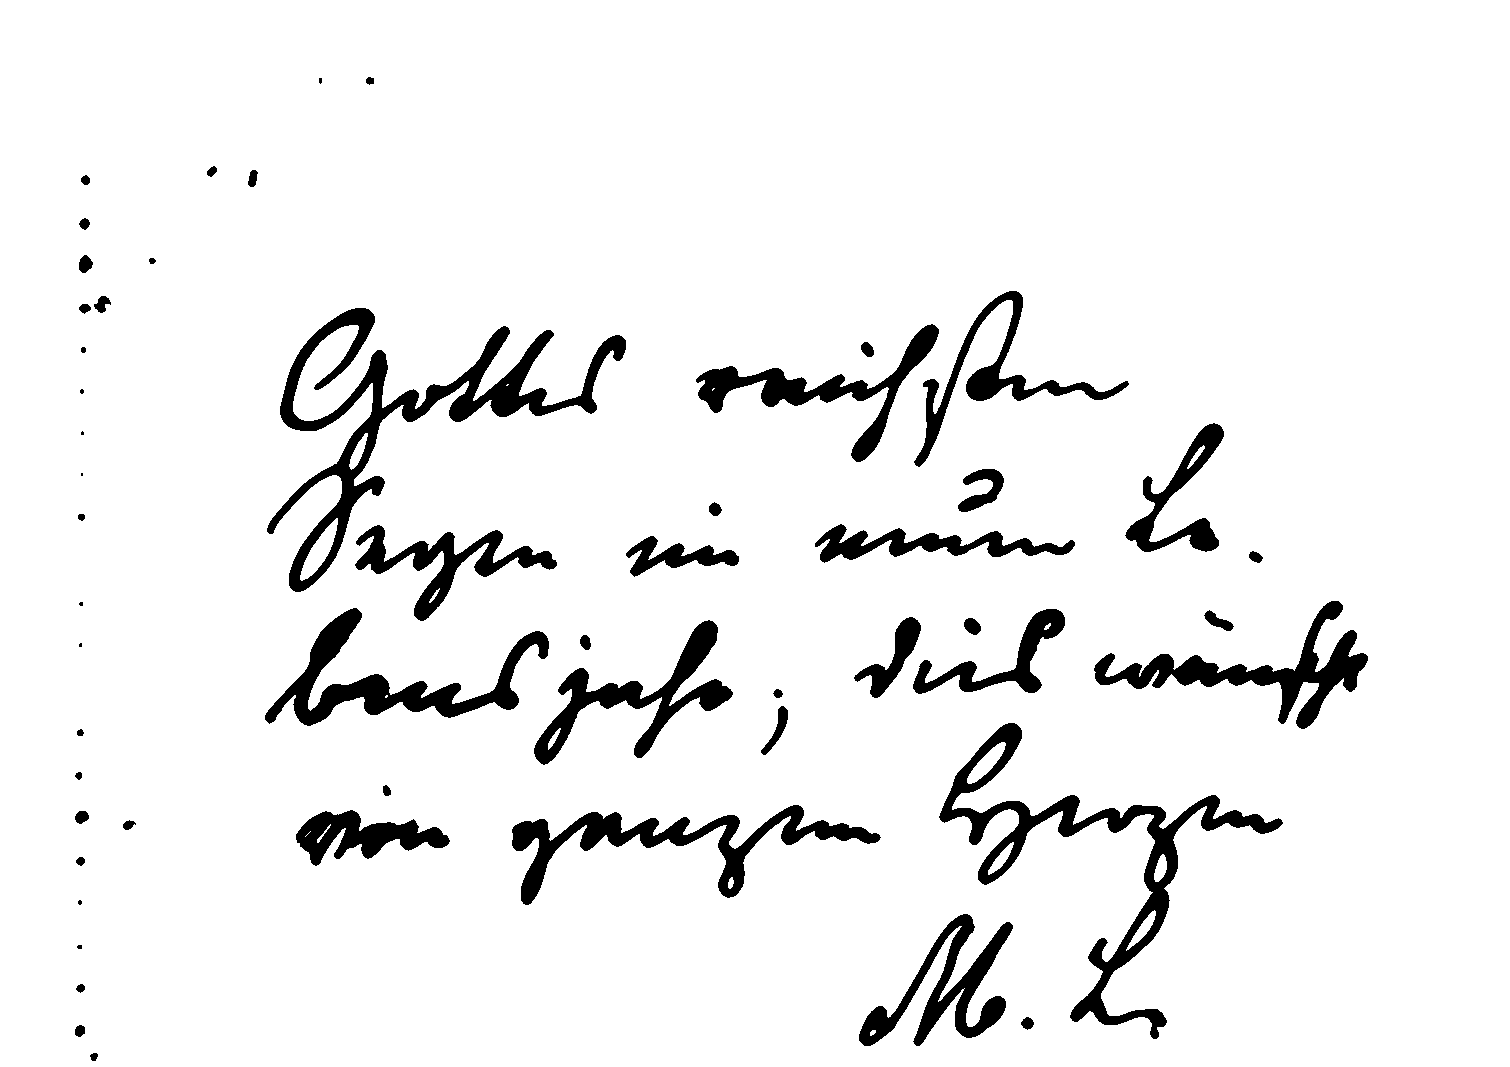
\includegraphics[width=8cm]{output.png}
    \caption{Original vs Final Binarized Image}
    \label{fig:7}
\end{figure}

\newpage

\section{Development Lifecycle}
The project lifecycle consisted of four main phases that were inherently
interwoven and iterated.

\subsection{Context}
The logical positivism research paradigm was well suited for this study since
it relies on the acquisition of material text documents that have certain
measurable objective properties. These properties include the textual content
of the documents as well as the associated artefacts. Unwanted artefacts and
degradation can therefore be viewed deterministically i.e., there are external
factors that produce these artefacts and an understanding of them can be used
to shape empirical models. By using scientific methods such as mathematical and
statistical analysis, empirical modelling and experimentation one can analyse
the documents and model their properties and dependent factors. The research
was viewed and planned through this philosophical perspective.\par

\subsection{Comprehension}
This phase was aimed at acquiring a firm understanding of the research question
and the context surrounding it. This required in-depth research on what
Document Image Binarization composes and which related topics needed to be
explored.

\subsection{Literature Study}
This phase was the longest and consisted of the exploration of different
approaches and solutions to the problems and ideas identified in the previous
phase. This also included research on supporting architecture, development
platforms, resources and environments in which the research would be conducted
and the artefact would be developed.

\subsection{Existing Solutions}
Once a firm understanding of the field was established, existing solutions were
researched and evaluated. This meant discovering and evaluating different
variations on the ideas previously identified.

\subsection{Development}
Candidate methods, ideas and technologies were identified and appropriate
open-source libraries were leveraged where needed. Several methods were
implemented, tested and relinquished.

\subsection{Iterative Approach}
Although the main lifecycle of the development of the project was sequential,
the phases were interlinked and were iterated and improved upon during the
entire span of this project.

\newpage

\section{Development of the Artefact}
\subsection{Comprehension}
This phase delivered a good grasp of the topics in general image processing, as
well as specific ideas and solutions for binarizing document images. Two main
sources were identified namely~\cite{su2012robust} and
~\cite{gatos2006adaptive} that each provided a functionally distinct scheme for
binarizing document images. These sources functioned as groundwork for further
topic exploration.

\subsection{Literature Study (Candidate Concepts)}
This subsection will outline the candidate concepts and ideas in image
processing and which problems they solve. These concepts were all implemented
and evaluated, but only the most viable solutions were selected.

\subsubsection{Denoising}
\paragraph{Wiener Filter}
The Wiener filter is optimal by the mean squared error measure since it is
defined by it. This property along with popular use and consistency of results
by ~\cite{6524379}, ~\cite{gatos2006adaptive} makes the wiener filter as well
as wavelet filters the obvious choice as candidates for denoising the document
images.
\par
~\cite{gatos2006adaptive} describes the use of an adaptive wiener filter that makes use of the local properties in an image to reduce noise using the following formula:
\[I(x,y)=\mu+\frac{(\sigma^2-v^2)(I_{source}-\mu)}{\sigma^2}\]
where \(\mu\) is the local mean, \(\sigma^2\) the variance in a 3 x 3 window
and \(v^2\) is the average variance.
\par
The selected algorithm is a variation on the original Wiener filter, called the
Wiener-Hunt filter that transforms the image into the frequency domain first by
using the Fourier transform
\[\hat x = F^\dagger (|\Lambda_H|^2 + \lambda |\Lambda_D|^2)
    \Lambda_H^\dagger F y\]
with \(F\) and \(F^\dagger\) the Fourier and inverse Fourier transforms
respectively, \(\Lambda_H\) the Fourier transform of the transfer function and
\(\lambda\) a damping constant as described by~\cite{scikit-image}.

\paragraph{Wavelet Filter}
The wavelet transform decomposes the image into a collection of wavelets. A
wavelet is a wave-like function, that has a finite 'energy' and a symmetric
area around the x-axis. The transform can be interpreted as the convolution of
a set of wavelets over the image that will output a signal proportional to the
similarity between the wavelets and the image.
\[ \int_{-\infty}^{\infty} f(x,y) \mathbf{\cdot} g(x,y) \,dx \]

Each wavelet has an associated scaling coefficient that acts as a thresholding
value, therefore, the selection of this thresholding value can be either
locally or globally based. The local methods are adaptive. The available
methods for calculating the scaling coefficients are BayesShrink and
VisuShrink. BayesShrink is an adaptive method that computes different
thresholds for each wavelet sub-band by using a Bayesian shrinkage estimator.
The Bayesian shrinkage estimator is a function that is inferred by using local
statistics of the image. This function determines the threshold for its
corresponding wavelet sub-band. VisuShrink calculates a single universal
threshold that determines every wavelet coefficient. The BayesShrink performed
the best on the widest range of images.\par

Other Denoising methods were considered such as total-variation denoising and
bilateral denoising.

\subsubsection{Morphological Filters}
Morphological filters determine the value of every pixel in the image using
some function of the pixels in a neighbourhood of the pixel.

\paragraph{Maximum Filter}
The maximum filter sets the value of a pixel to the maximum intensity value of
the pixels in a neighbourhood of the pixel.

\paragraph{Minimum Filter}
The maximum filter sets the value of a pixel to the minimum intensity value of
the pixels in a neighbourhood of the pixel.\par

By combining these filters, we can obtain the opening and closing filters.

\paragraph{Opening Filter}
The opening filter is composed of combining the application of the maximum
filter followed by the minimum filter. The opening filter is used to remove
small objects in the image while preserving the more prominent larger objects.
By setting the window size equal to the estimated average stroke width of the
text in the image, This filter removes specks and other small defects in the
image while preserving the text.

\paragraph{Closing Filter}
The closing filter is composed of combining the application of the minimum
filter followed by the maximum filter. The closing filter is used to smooth
images. This filter is not of much use in this context.

\paragraph{Mean Filter}
The mean filter sets the value of a pixel to the arithmetic mean intensity
value of the pixels in a neighbourhood of the pixel. This filter is not of much
use in this context since it is used for blurring an image.

\paragraph{Median Filter}
The median filter is similar to the previous filters in that it is non-linear,
but this filter is very popular and useful since it preserves edges while
removing noise. The median filter sets the value of a pixel to the median
intensity value of the pixels in a neighbourhood of the pixel. This filter
could be used as an alternative to some of the other image-denoising
techniques.

\subsubsection{Edge Detection}
Although edge detection is a higher-level process used mostly by processes
further along in the image processing pipeline, there are a few reasons why
edge detection is beneficial. Edge detection can be used for image segmentation
and text stroke width estimation. Since most edge detection methods rely on
some sort of gradient function, there is the added benefit of noise removal in
areas with low contrast or high-frequency pixel intensities (noise).

\paragraph{Variance}
Since variance is a measure of dispersion or variability, areas with high
variance in intensity values such as the edges of the text are highlighted by
implementing a variance filter. The downside of the variance measure is that
data can be arbitrarily widespread, thus the variance is unbound and can behave
unpredictably.

\paragraph{Prewitt operator}
The Prewitt operator uses two 3x3 kernels which are convolved with the image to
calculate approximations of the directional derivatives.
\[\mathbf{G}_x=\begin{bmatrix}
        1 & 0 & -1 \\
        2 & 0 & -2 \\
        1 & 0 & -1 \\
    \end{bmatrix} and
    \mathbf{G}_y=\begin{bmatrix}
        1  & 2  & 1  \\
        0  & 0  & 0  \\
        -1 & -2 & -1 \\
    \end{bmatrix}
\]

By calculating the magnitude and angle of the resulting images one can obtain
information about the direction of lines in the image.

\paragraph{Sobel operator}
The Sobel operator is similar to the Prewitt operator.
\[\mathbf{G}_x=\begin{bmatrix}
        1 & 0 & -1 \\
        1 & 0 & -1 \\
        1 & 0 & -1 \\
    \end{bmatrix} and
    \mathbf{G}_y=\begin{bmatrix}
        1  & 1  & 1  \\
        0  & 0  & 0  \\
        -1 & -1 & -1 \\
    \end{bmatrix}
\]

\paragraph{Canny Edge Detector}
The Canny edge detection algorithm works as follows:
\begin{enumerate}
    \item A Gaussian filter is convolved to remove noise.
    \item The intensity gradient of the image is calculated by using directional edge
          operators such as Roberts, Prewitt or Sobel.
    \item The gradient magnitude is calculated and used as an upper and lower threshold
    \item Track edges by hysteresis.
\end{enumerate}

~\cite{rong2014improved} outlines the principal part of the algorithm where the edges are identified by calculating the gradient between pixels. The following first-order partial derivative estimations are used on the original image \(I\) for pixels \(i,j \in I\):

\[E_x(i,j)=\frac{1}{2}(I(i+1,j)-I(i,j)+I(i+1,j+1)-I(i,j+1))\]
\[E_y(i,j)=\frac{1}{2}(I(i,j+1)-I(i,j)+I(i+1,j+1)-I(i+1,j))\]
which can also be written in matrix form as
\[\mathbf{G}_x=\begin{bmatrix}
        -1 & 1 \\
        -1 & 1 \\
    \end{bmatrix},
    \mathbf{G}_y=\begin{bmatrix}
        1  & 1  \\
        -1 & -1 \\
    \end{bmatrix}
\]

The magnitude is calculated as
\[|\mathbf{G}|=\sqrt{\mathbf{G}_x^2+\mathbf{G}_y^2}\]
and the edge direction as
\[\Theta=atan2(\mathbf{G}_y,\mathbf{G}_x)\]

~\cite{rong2014improved}identifies some problems with the traditional Canny algorithm. The first is that since the convolution window is a 2x2 matrix, it is sensitive to noise. Seeing that the algorithm uses the partial derivatives in the x and y direction, it is not sensitive to edges oriented $90^{\circ}$ relative to the major axes.\par

Due to this, some augmented methods have been constructed that attempt to solve
these issues such as those proposed by~\cite{rong2014improved}
and~\cite{xuan2017improved}

By calculating the magnitude and angle of the resulting images one can obtain
information about the direction of lines in the image.

\paragraph{Gradient Image}
The technique used by~\cite{su2012robust} requires the generation of a contrast
image for stroke width detection. An image is constructed using a formula for
identifying local image contrast:
\begin{equation}
    \label{E:4}
    C(i,j)=\frac{I_{max}(i,j)-I_{min}(i,j)}{I_{max}(i,j)+I_{min}(i,j)+\epsilon}
\end{equation}
where \(\epsilon\) is a positive infinitesimal. The denominator scales the input according to the local range of values, thereby normalizing the contrast across the image~\cite{su2012robust}. Next, a constant \(a\) is calculated:
\begin{equation}
    \label{E:5}
    a=(\frac{\sigma}{128})^\gamma, \; \gamma \geq 0
\end{equation}
\(\sigma\) is the standard deviation of the entire document image intensities.
By combining \ref{E:1} and \ref{E:2} we derive the final equation they use to construct the Gradient image:
\begin{equation}
    \label{E:6}
    C_a(i,j)=a\times C(i,j)+(1-a)(I_{max}(i,j)-I_{min}(i,j))
\end{equation}
Which results in
\begin{figure}[htp]
    \centering
    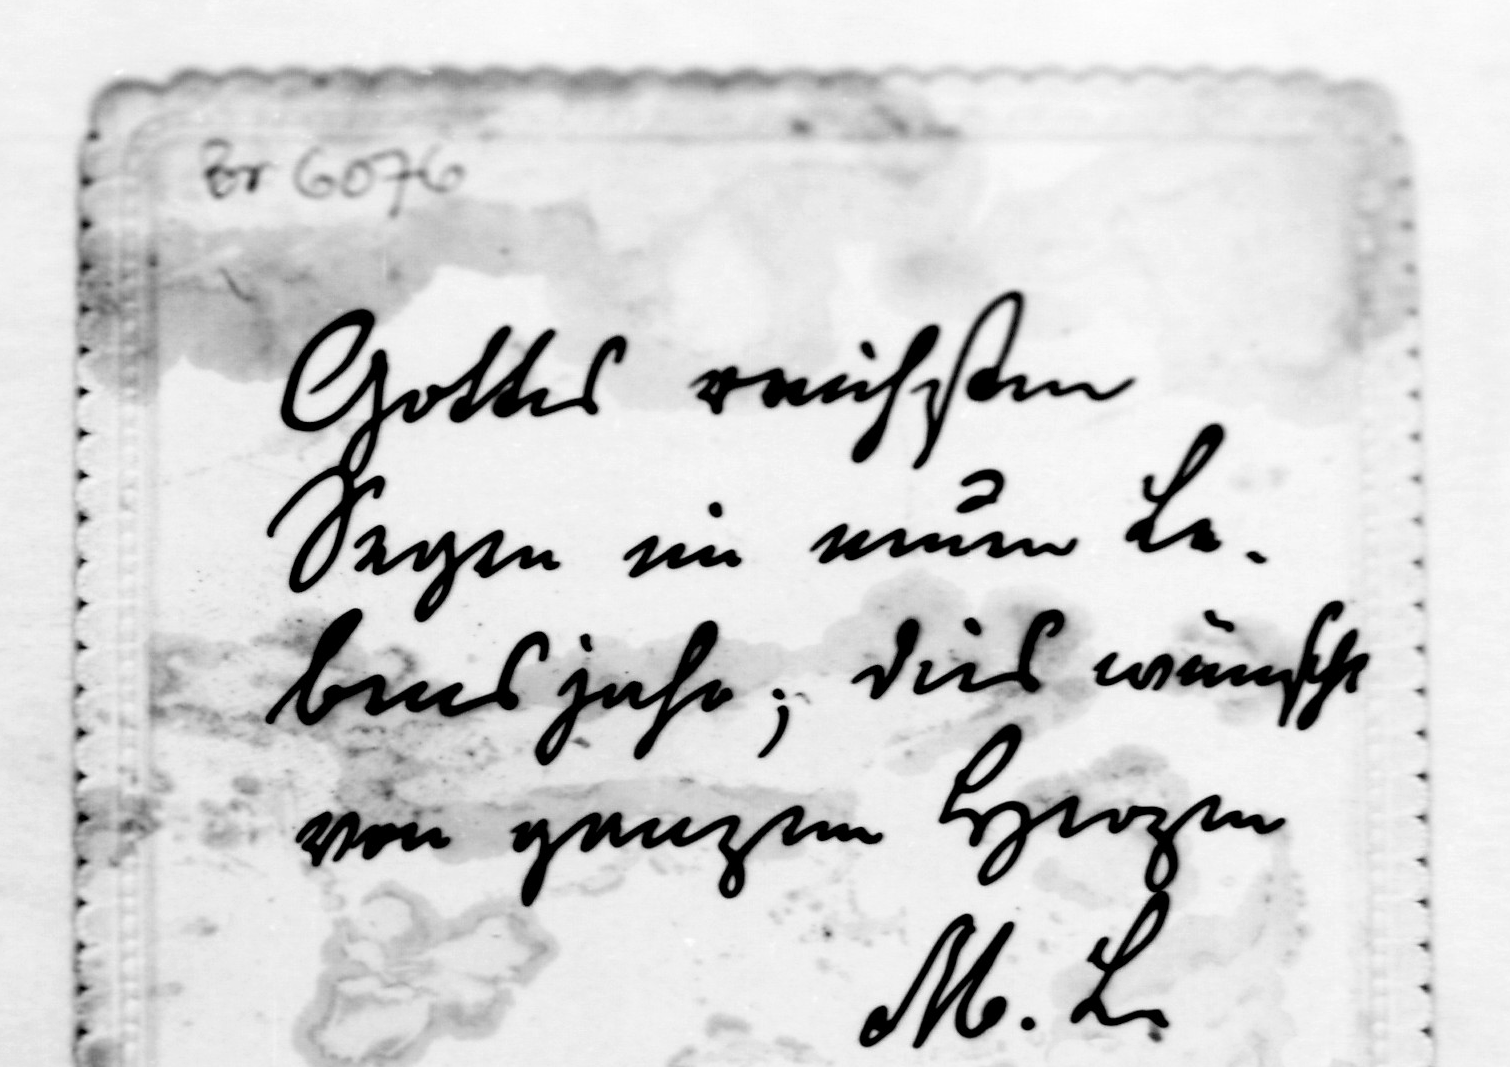
\includegraphics[width=4cm]{original.png}
    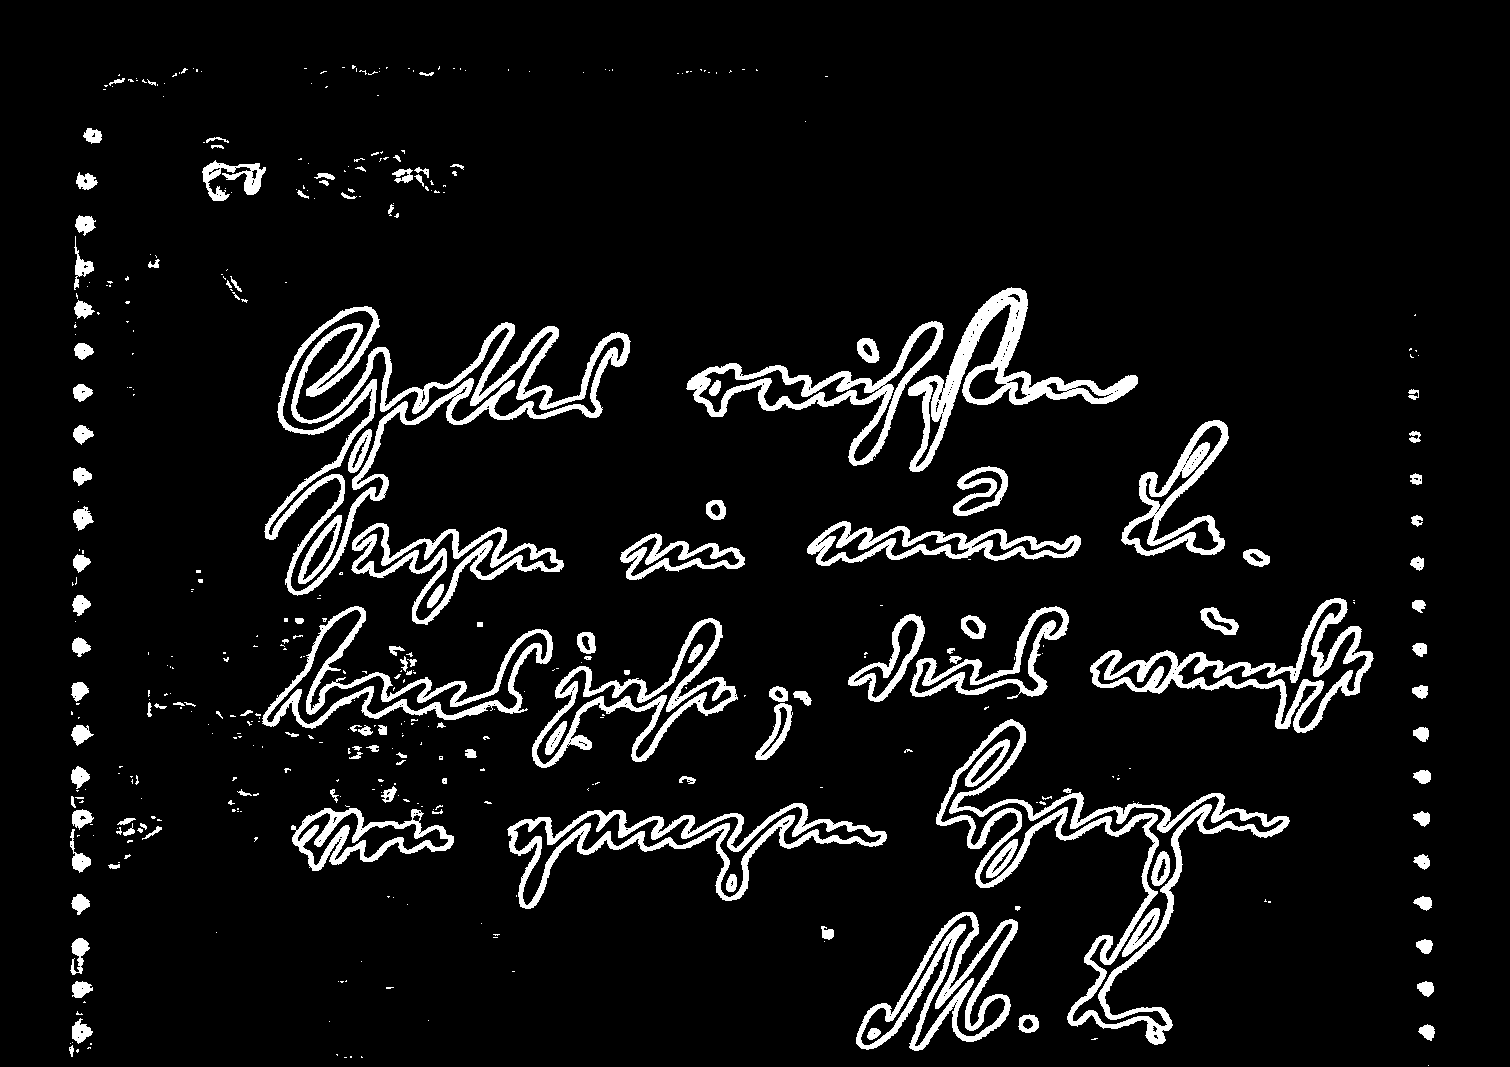
\includegraphics[width=4cm]{contrast-image.png}
    \caption{Original Document Image and Contrast Image}
    \label{fig:contrast}
\end{figure}

\subsubsection{Thresholding}

\paragraph{Sauvola's Method}
The Sauvola local thresholding method calculates a threshold $T$ in every
neighbourhood around every pixel in the image~\cite{scikit-image}. This method
is an adaptation of Niblack's method. This is also the thresholding method used
by~\cite{gatos2006adaptive}.
\[T=\mu*\frac{R+k*(\sigma-R)}{R}\]
where a chosen $k$ scales the standard deviation parameter $\sigma$

\paragraph{Otsu's Method}
Otsu's method is an automatic image thresholding approach. The algorithm
returns a single intensity threshold, dividing pixels into the foreground and
background classes. This threshold is calculated by optimising for inter-class
and intra-class variance. The algorithm uses an exhaustive search for the
threshold parameter that minimises the intra-class variance defined as:
\[\sigma_{\omega}^{2}(t)=\omega_0(t)\sigma_0^2(t)+\omega_1(t)\sigma_1^2(t)\]
with $\omega_0$ and $\omega_1$ the probabilities and $\sigma_0^2$ and
$\sigma_1^2$ the variances of the mutually exclusive classes. The threshold is
then selected as the maximum value of $\sigma_{\omega}^{2}$.

\subsubsection{Stroke Width Estimation}
An estimation of text stroke width will be utilised in the final step. An
effective method of doing this as introduced by~\cite{strokewidth} consists of
two main steps, namely performing a distance transform and then skeletonizing
the image.

\paragraph{Distance Transform}
The distance transform uses the thresholded image and assigns each pixel a
value according to its euclidean distance to the closest white pixel
(background pixel), thereby creating an image with the brightest pixels in the
centre of the text.

\paragraph{Skeletonizing}
Skeletonizing an image consists of making multiple passes over an image and
detecting the edge pixels. These edge pixels are then removed unless they break
the connectivity of the identified object~\cite{scikit-image}. The implemented
method is the Zhang adaptation~\cite{zhang_suen_1984} that traverses the image
and removes the boundary and corner points of foreground sections. Doing this
iteratively leaves only a 1-pixel-wide skeleton.

Since the pixels in the middle of each stroke are the furthest away from the
background pixels and the skeletonized image contains white pixels only in the
centres of the stroke, the indexes of the foreground (bright) pixels in the
skeletonized image are iterated in the distance-transformed image. The selected
pixel values in the distance-transformed image are summed and averaged to
obtain a quantity half of the actual average text stroke width since it
measured the distance from the centre of the stroke to the edge of the stroke,
therefore half of the actual width.

\subsubsection{Development Platforms and Environments}

\paragraph{Programming Language}
The selected programming language needed:
\begin{itemize}
    \item Comprehensive libraries in support of a wide variety of image processing
          concepts.
    \item Comprehensive, comprehensible documentation of the language and relevant
          libraries.
    \item Integration with technologies that may make use of the artefact
    \item To be suitable for processing images.
    \item To be effective for prototyping and testing.
\end{itemize}

These constraints were satisfied in the Python and C++ programming languages
with libraries such as OpenCV in both languages and additionally python
libraries such as \href{https://numpy.org/}{numpy},
\href{https://scikit-image.org/}{scikit-image} and
\href{https://scikit-image.org/}{scipy}.\par

Both languages were tested. Python was easy to understand and use, but since it
is a dynamically typed language debugging was difficult and inefficient. The
processing of images is also a highly intensive task, which made the slow
execution speed of python scripts noticeable and hindering. The decision was
made to switch to C++, but difficulty importing libraries and slow development,
prototyping and testing led to the switch back to Python.\par

In the end, Python was suitable for the development and testing of the
artefact.

\paragraph{Front-end application}
Proficient experience in the Angular web framework resulted in it becoming the
obvious choice for testing and interfacing with the artefact. This application
was very simple and only had the purpose of displaying the test images and the
results.

\paragraph{Middelware}
The front-end application needed a way to run the Document Image Binarization
script. The Node.js JavaScript runtime was selected to serve and run the script
since the \href{https://expressjs.com/}{Express}~\cite{express} library makes
this process very simple.

\chapter{Results}
By applying the proposed method to a range of 10 images provided by
\href{https://vc.ee.duth.gr/h-dibco2016/}{DIBCO 2016 Handwritten
    DocumentDataset}, we get the following results:

\begin{table}[]
    \centering
    \begin{tabular}{>{\columncolor[HTML]{C0C0C0}}l |llll}
        \cellcolor[HTML]{C0C0C0}                &
        \cellcolor[HTML]{C0C0C0} Input Image    &
        \cellcolor[HTML]{C0C0C0} Output Image     \\
        \hline
        {\color[HTML]{FFFFFF} }                 &
        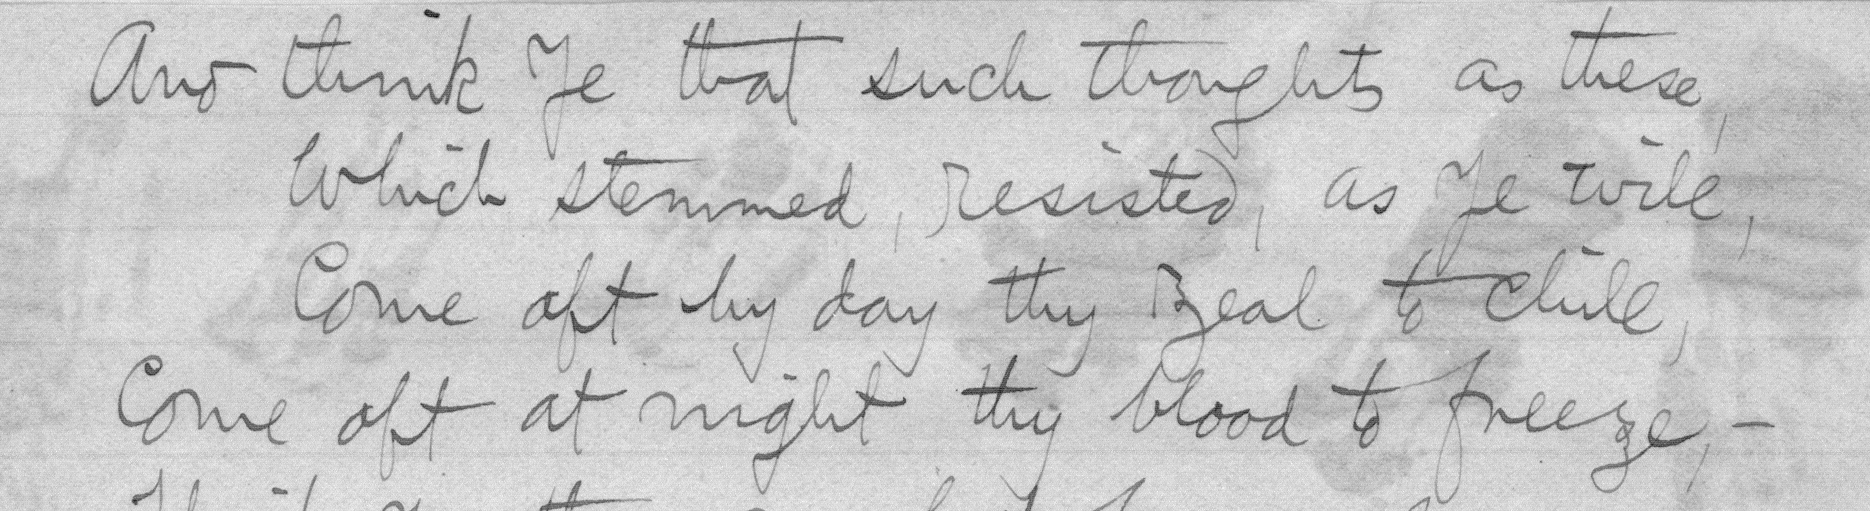
\includegraphics[width=8cm]{3input.png} &
        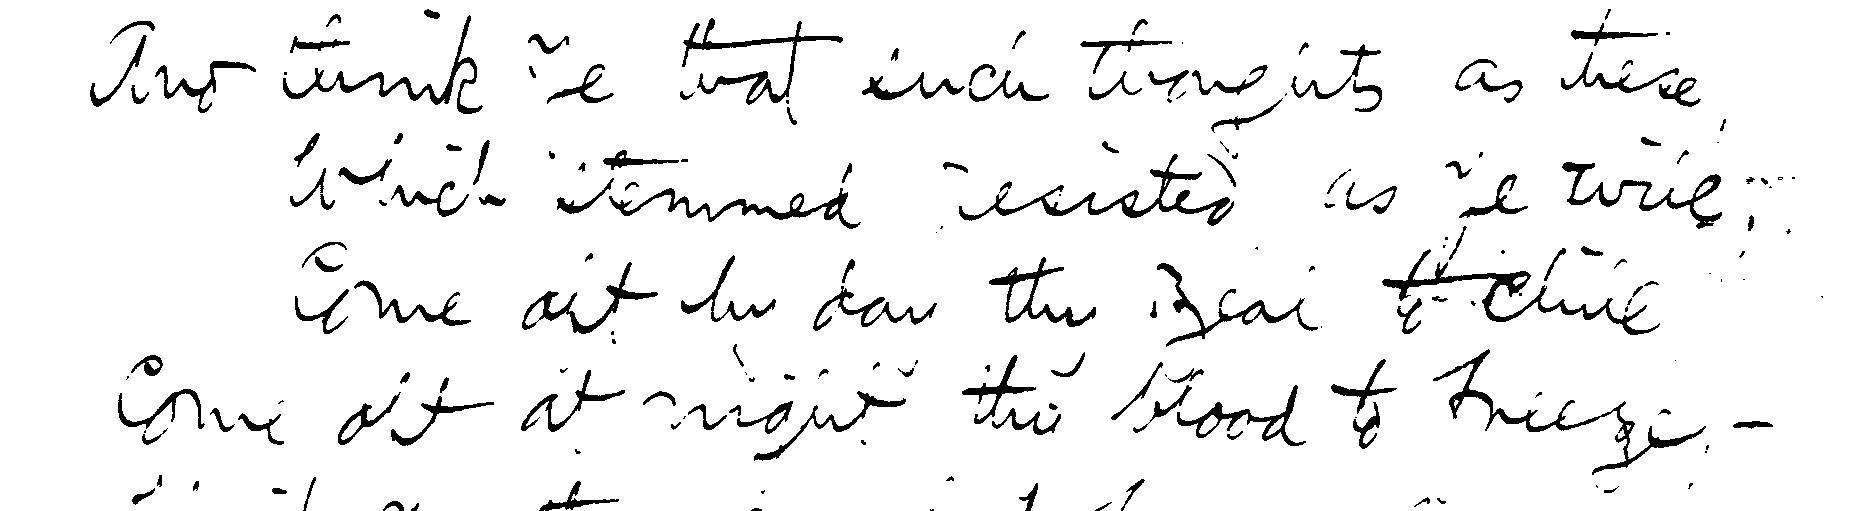
\includegraphics[width=8cm]{3output.png}  \\
        \hline
        {\color[HTML]{FFFFFF} }                 &
        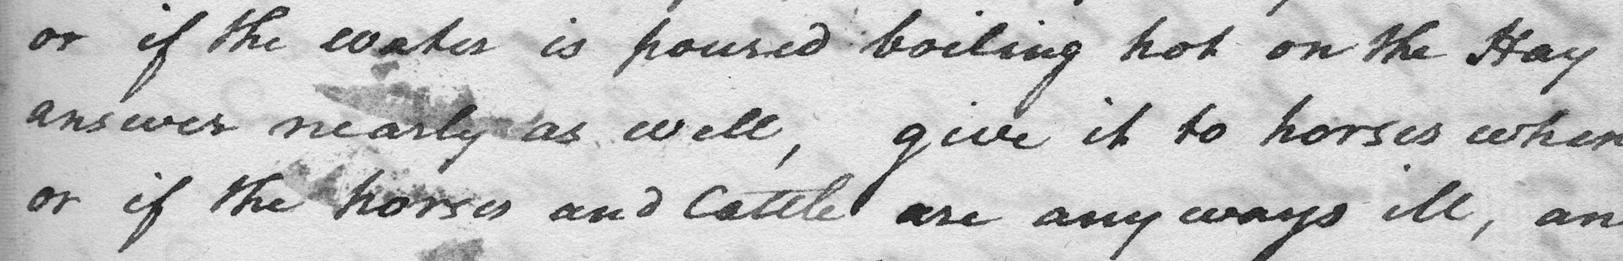
\includegraphics[width=8cm]{5input.png} &
        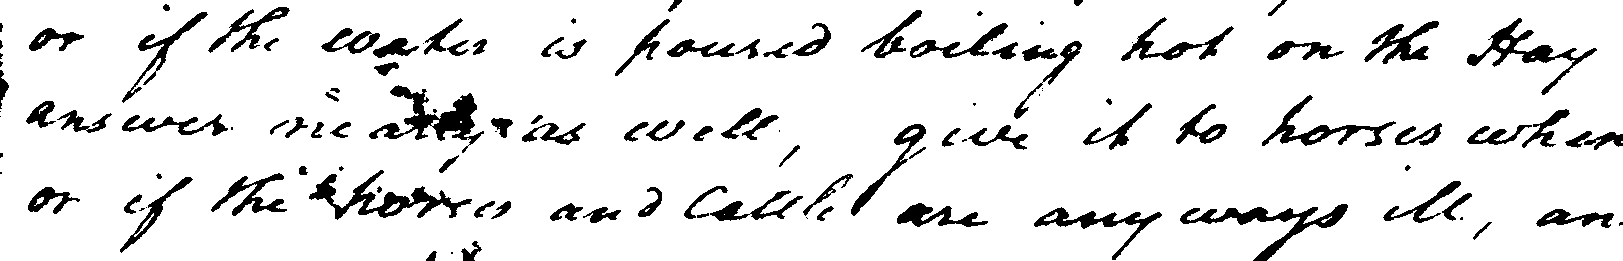
\includegraphics[width=8cm]{5output.png}  \\
        \hline
    \end{tabular}
\end{table}

\begin{table}[]
    \centering
    \begin{tabular}{>{\columncolor[HTML]{C0C0C0}}l |llll}
        \cellcolor[HTML]{C0C0C0}                 &
        \cellcolor[HTML]{C0C0C0} Input Image     &
        \cellcolor[HTML]{C0C0C0} Output Image      \\
        \hline
        {\color[HTML]{FFFFFF} }                  &
        
\includegraphics[width=8cm]{12input.png} &
        
\includegraphics[width=8cm]{12output.png}  \\
        \hline
        {\color[HTML]{FFFFFF} }                  &
        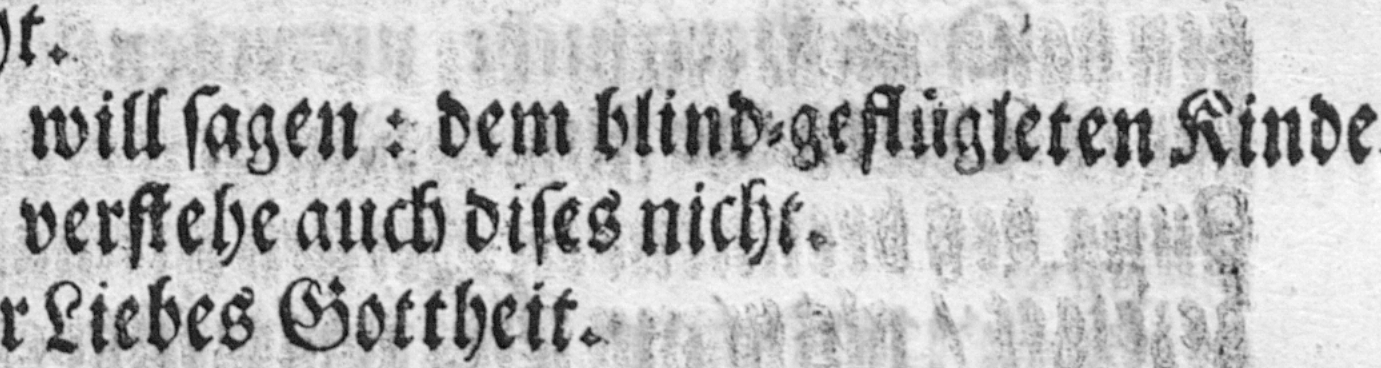
\includegraphics[width=8cm]{9input.png}  &
        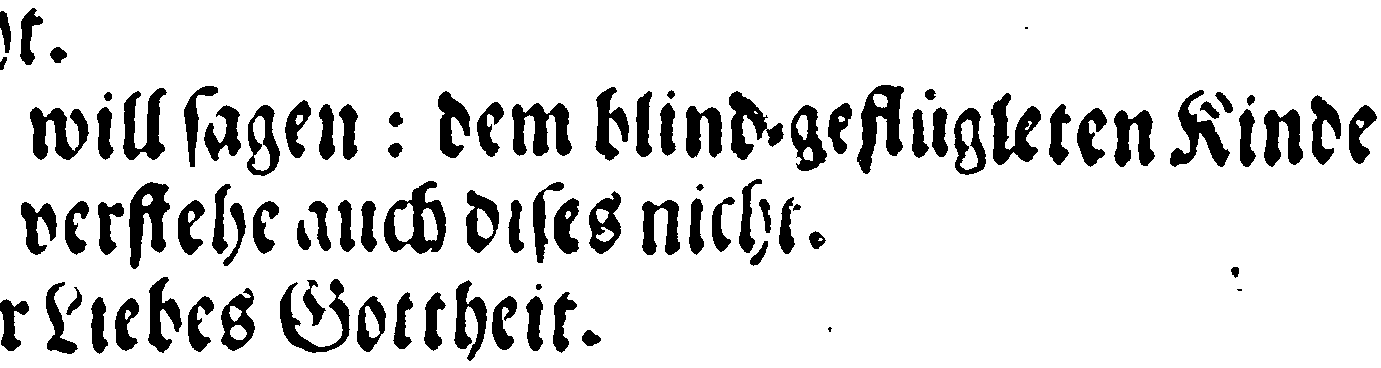
\includegraphics[width=8cm]{9output.png}   \\
        \hline
        {\color[HTML]{FFFFFF} }                  &
        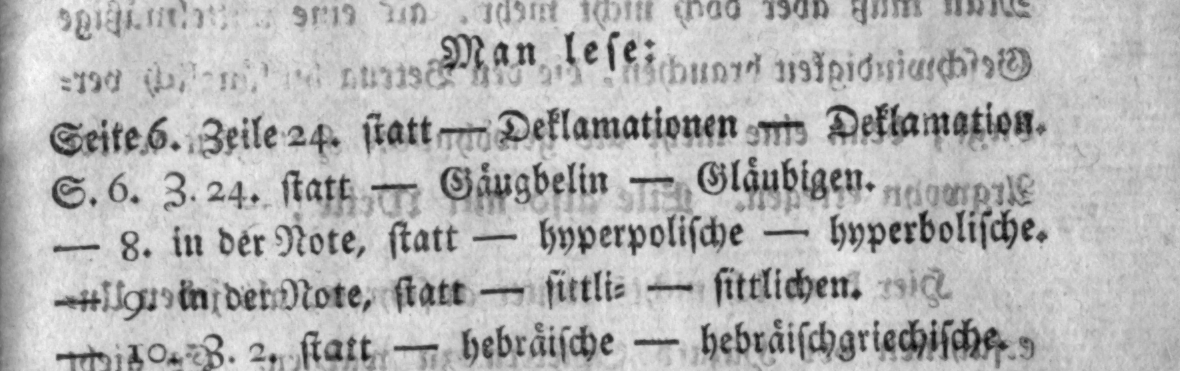
\includegraphics[width=8cm]{10input.png} &
        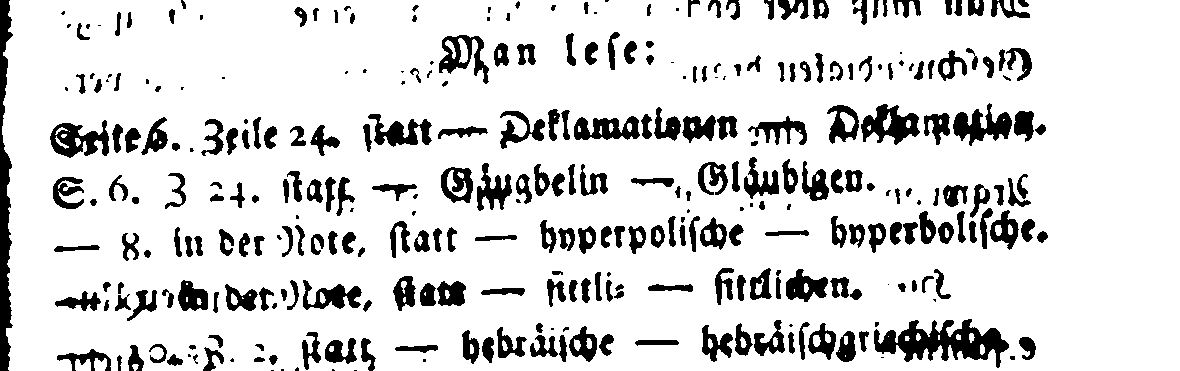
\includegraphics[width=8cm]{10output.png}  \\
        \hline
        {\color[HTML]{FFFFFF} }                  &
        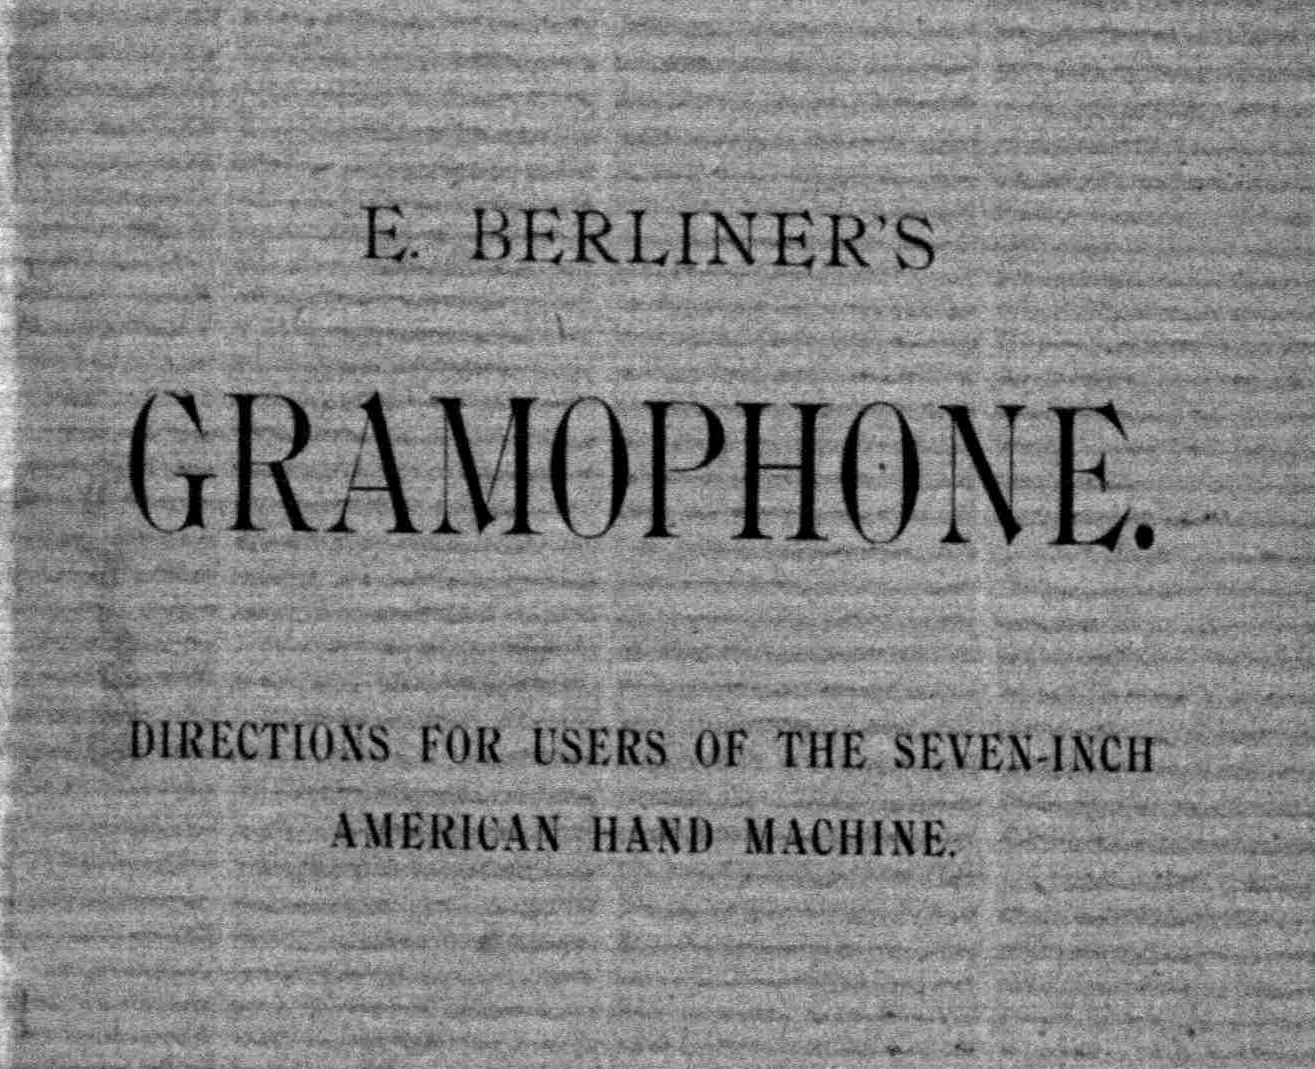
\includegraphics[width=8cm]{14input.png} &
        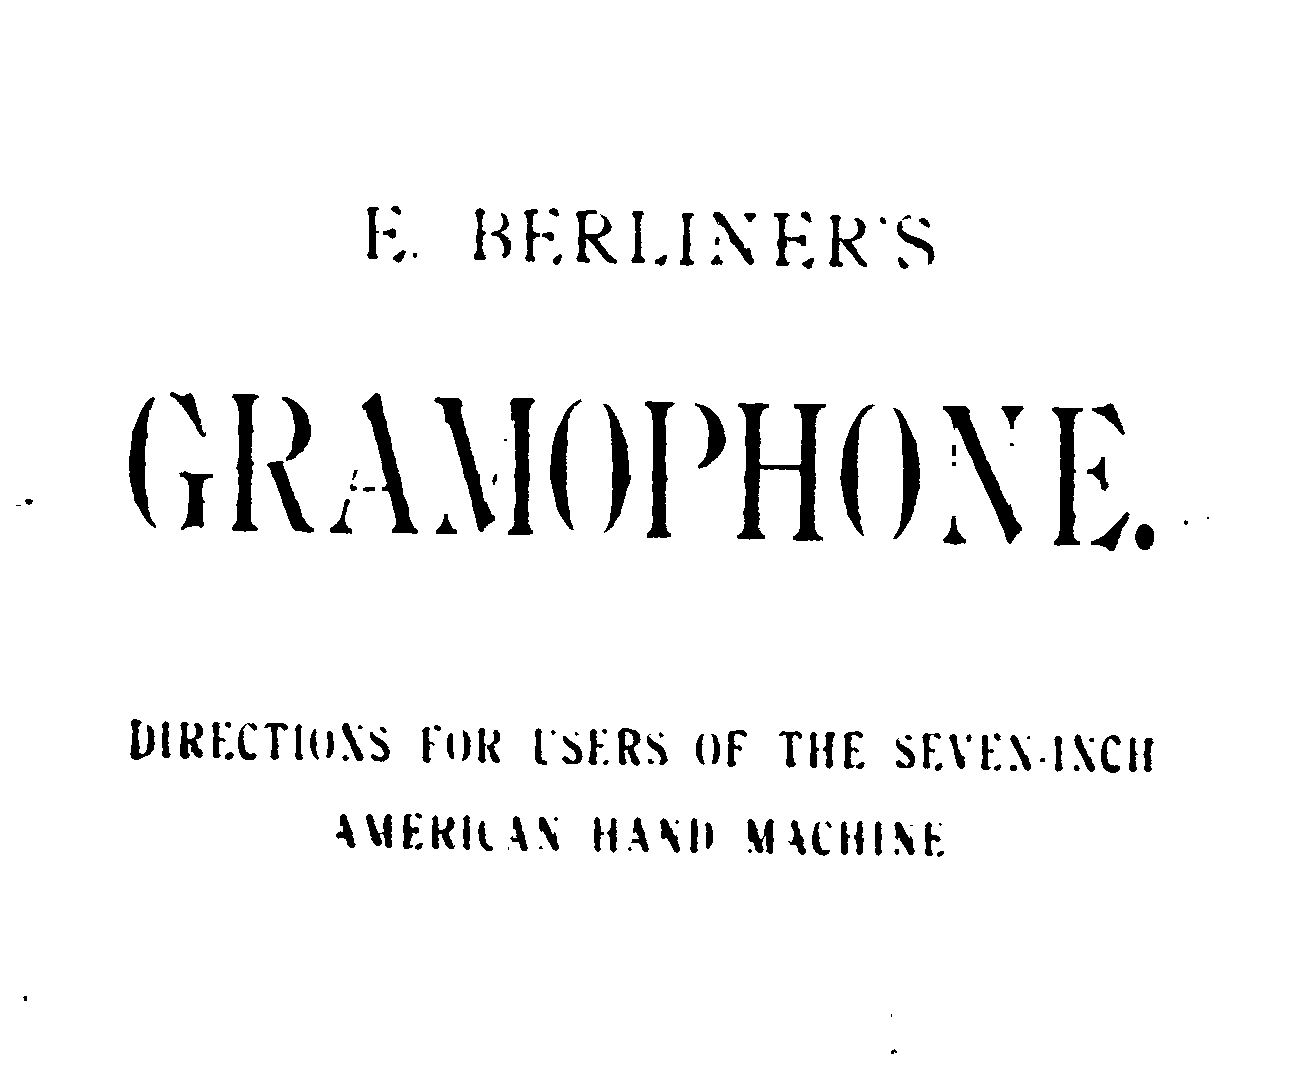
\includegraphics[width=8cm]{14output.png}  \\
        \hline
        {\color[HTML]{FFFFFF} }                  &
        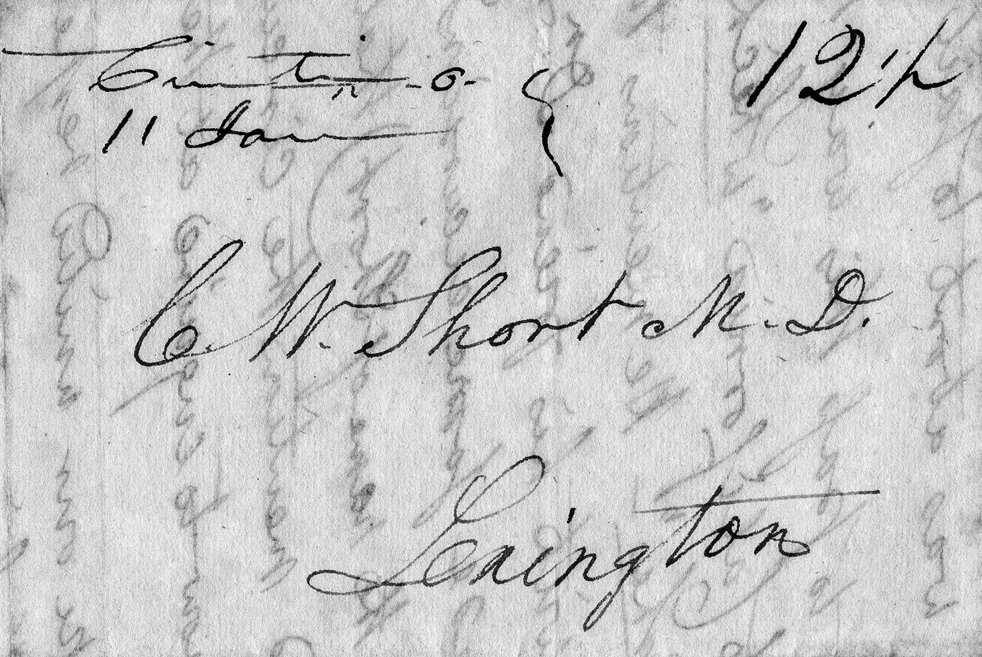
\includegraphics[width=8cm]{7input.png}  &
        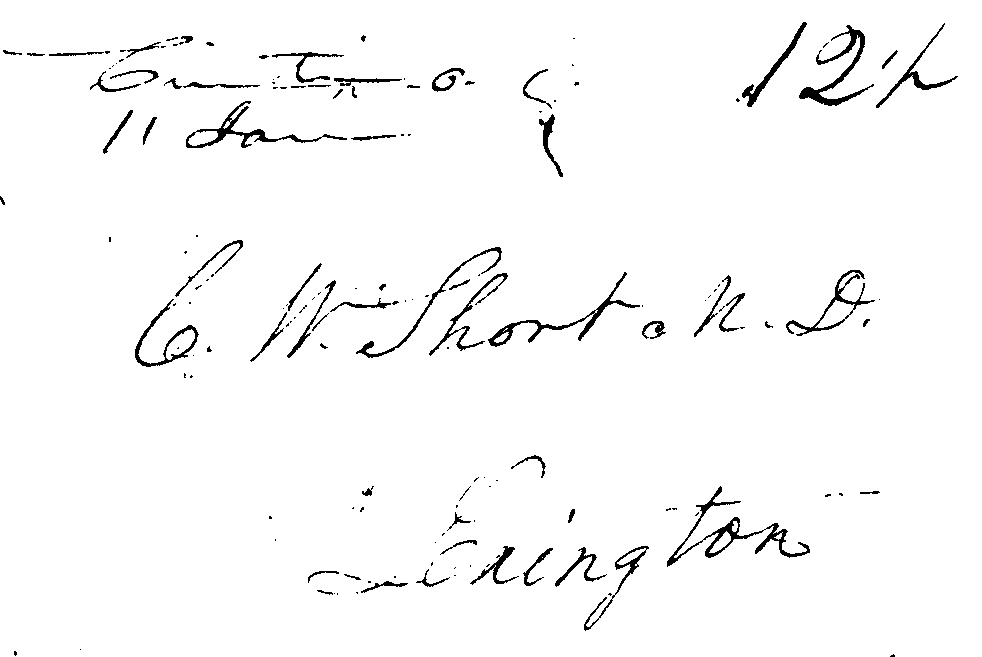
\includegraphics[width=8cm]{7output.png}   \\
    \end{tabular}
\end{table}

\begin{table}[]
    \centering
    \begin{tabular}{>{\columncolor[HTML]{C0C0C0}}l |llll}
        {\color[HTML]{FFFFFF} }                  &
        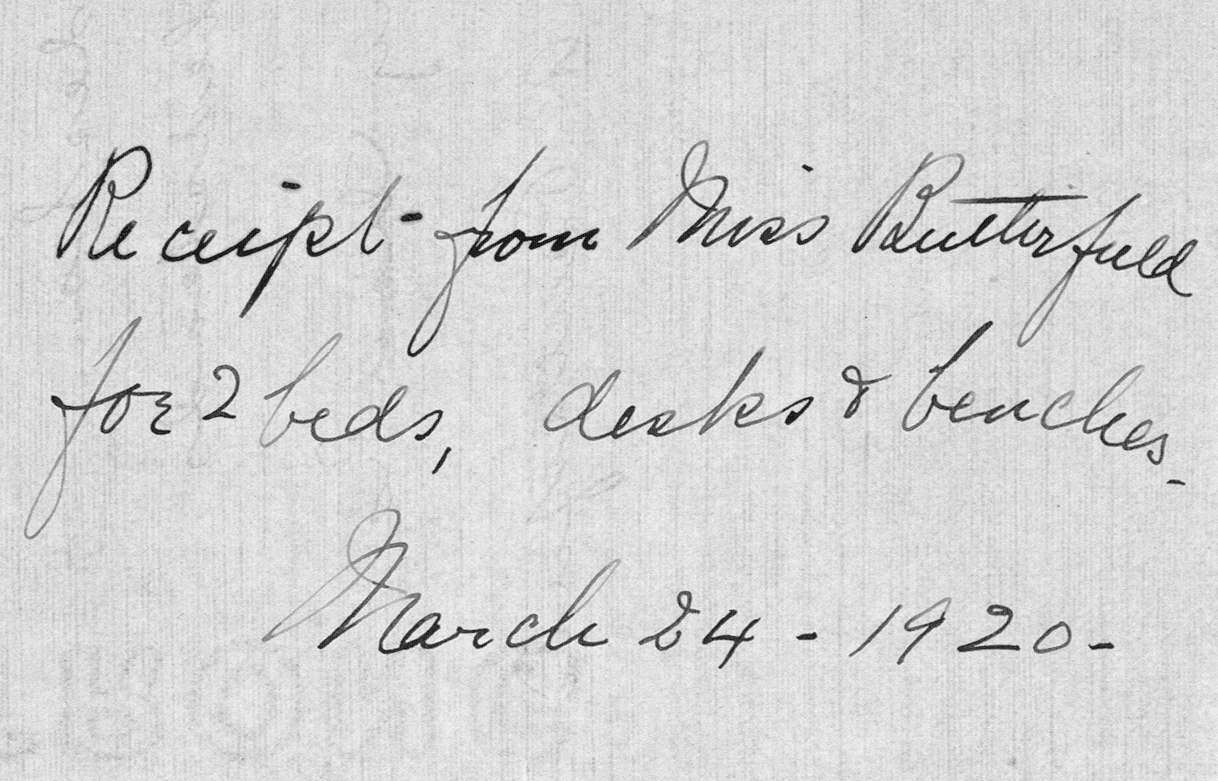
\includegraphics[width=8cm]{2input.png}  &
        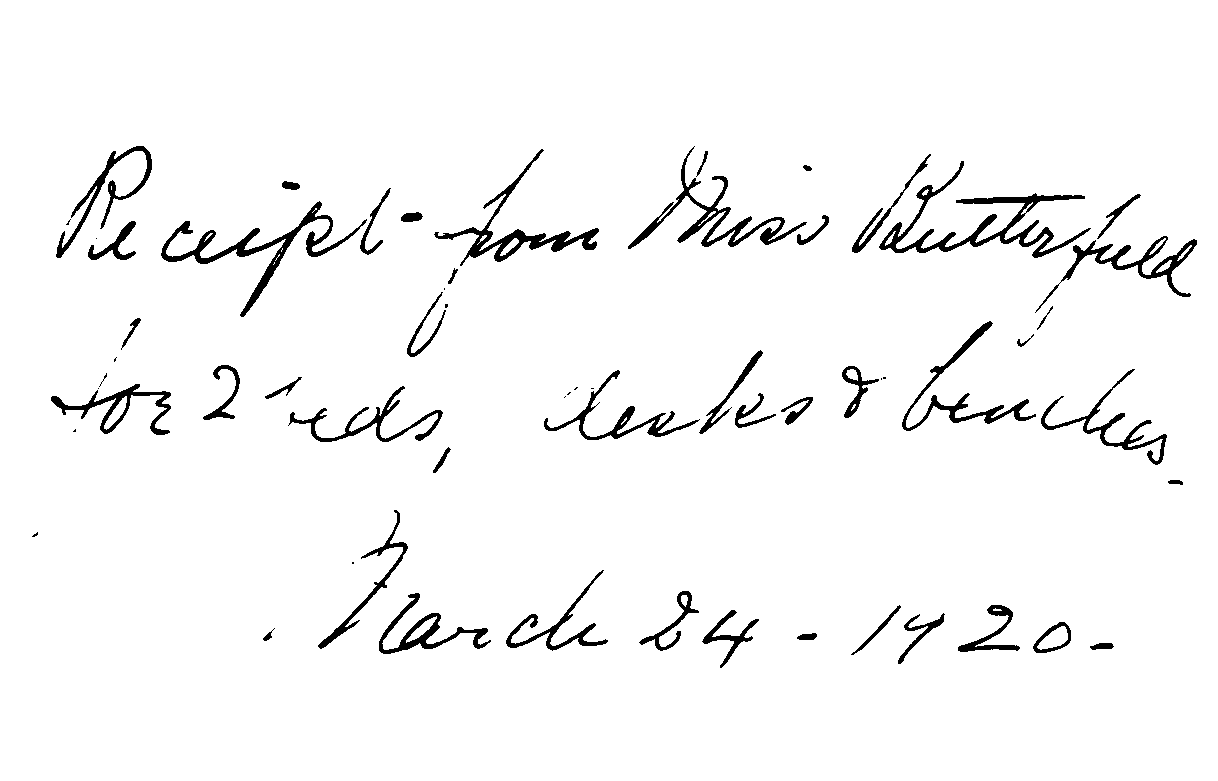
\includegraphics[width=8cm]{2output.png}   \\
        \hline
        {\color[HTML]{FFFFFF} }                  &
        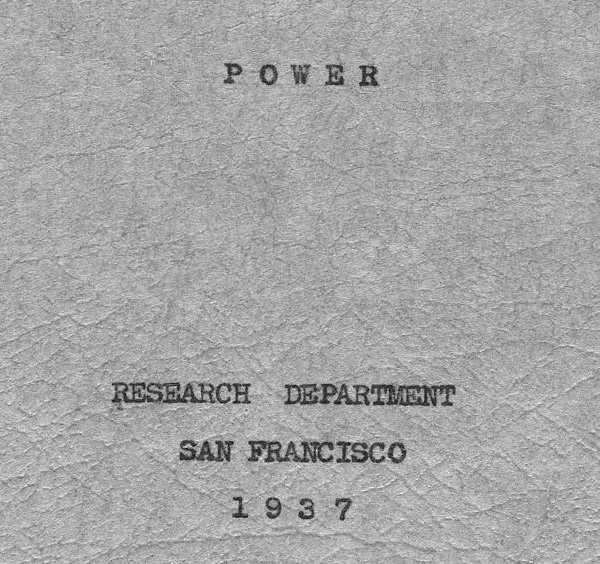
\includegraphics[width=8cm]{15input.png} &
        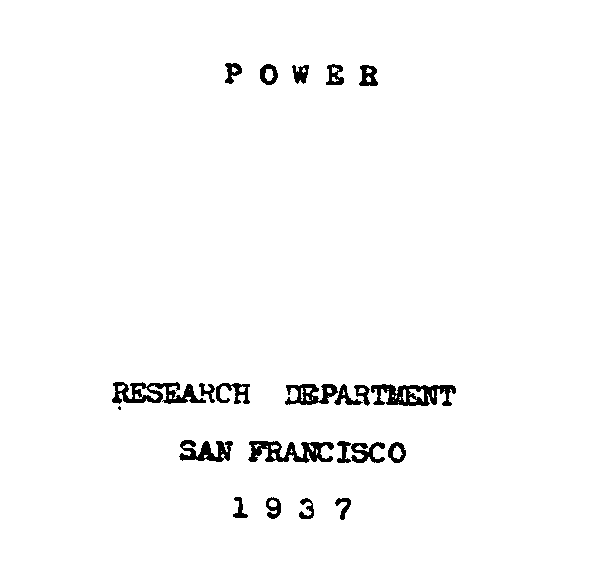
\includegraphics[width=8cm]{15output.png}  \\
        \hline
        {\color[HTML]{FFFFFF} }                  &
        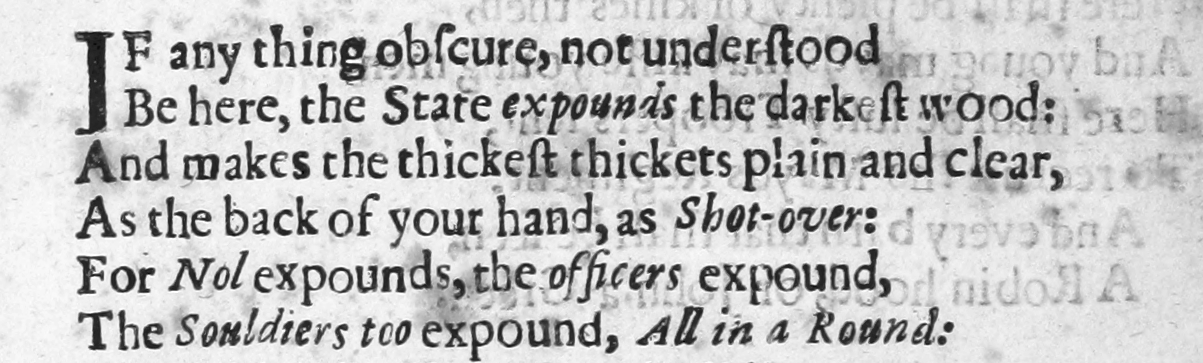
\includegraphics[width=8cm]{11input.png} &
        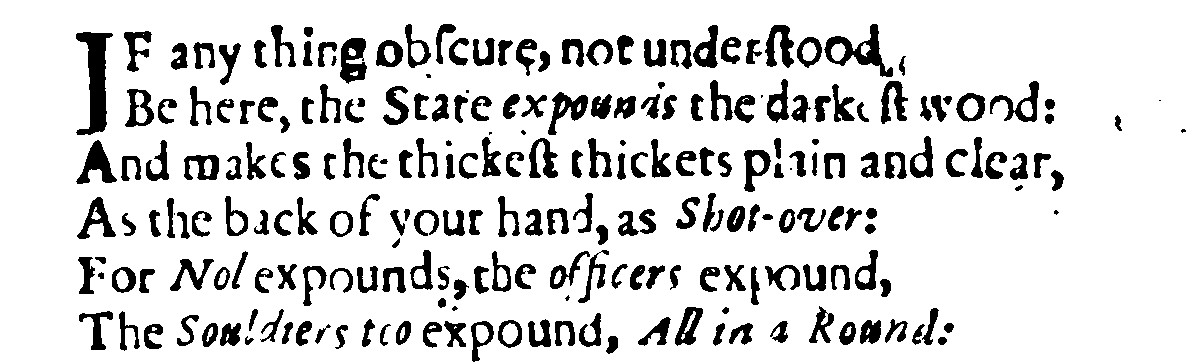
\includegraphics[width=8cm]{11output.png}  \\
    \end{tabular}
\end{table}

\chapter{Reflection}

\newpage
\printbibliography
\end{document}